\documentclass{article}

\usepackage[top=1in,bottom=0.5in,left=0.5in,right=0.5in]{geometry}
\usepackage{amsmath,amssymb,multirow,graphicx}

\newcommand{\bx}{\mathbf{x}}
\newcommand{\by}{\mathbf{y}}
\newcommand{\bn}{\mathbf{n}}
\newcommand{\bu}{\mathbf{u}}
\newcommand{\ff}{\mathbf{f}}
\newcommand{\phie}{\phi_{\epsilon}}
\newcommand{\psie}{\psi_{\epsilon}}
\newcommand{\vphie}{\varphi_{\epsilon}}
\newcommand{\eps}{\epsilon}

\newcommand{\bee}[1]{\begin{equation} #1 \end{equation}}
\newcommand{\baa}[1]{\begin{eqnarray} #1 \end{eqnarray}}
\newcommand{\bees}[1]{\begin{equation*} #1 \end{equation*}}
\newcommand{\baas}[1]{\begin{eqnarray*} #1 \end{eqnarray*}}


\newcommand{\dd}[2]{\ensuremath{\frac{\text{d} #1}{\text{d} #2}}}
\newcommand{\ddd}[2]{\ensuremath{\frac{\text{d}^2 #1}{\text{d} {#2}^2}}}
\newcommand{\pd}[2]{\ensuremath{\frac{\partial #1}{\partial #2}}}
\newcommand{\pdd}[2]{\ensuremath{\frac{\partial^2 #1}{\partial {#2}^2}}}
\newcommand{\pddd}[3]{\ensuremath{\frac{\partial^2 #1}{\partial #2 \partial #3}}}

\begin{document}
\section{Boundary element method in conjunction with regularized Stokeslets}

We are solving for the fluid flow around a steadily translating cylinder of radius $a=0.25$ in an infinite fluid with viscosity $\mu=1.0$. We use the 2D steady Stokes equations $\mu\Delta \bu(\bx) = -\nabla p$ with boundary conditions $\bu = [1,0]$ on the circle to approximate the solution near the cylinder. The exact solution to this test case for $r>0.25$ is a combination of a Stokeslet and a dipole at the origin:

\begin{eqnarray}\label{exactsoln}
	\bu(\bx) &=& \frac{-\ff_0}{8\pi\mu}\left( 2\ln\lvert\bx\rvert - a^2/\lvert \bx \rvert^2 \right) + \frac{\left(\ff_0 \cdot \bx \right)\bx}{4\pi\mu\lvert \bx \rvert^2}\left(1-a^2/\lvert \bx \rvert^2\right) \nonumber \\
	\ff_0 &=& \frac{8\pi}{1-2\ln(a)}\begin{pmatrix} 1 \\ 0 \end{pmatrix}.
\end{eqnarray}
	
We have previously solved this problem using a regularization method on the singular kernel in the boundary integral equation. That method, as pointed out by Smith (2009), uses a Riemann sum approximation to perform integration. He proposes using a boundary element method (BEM) to reduce the size of the matrix needed to solve the integral equation numerically. We seek to compare these methods.

As a test case we will consider the $L_2$ norm of the error over two patches of points, one close to the circle and one farther away as in Fig. \ref{schematic}. The patches are square with five equally spaced points in between $0.48$ and $0.50$ in the far patch and between $0.255(\cos(\pi/4),\sin(\pi/4))$ and $0.255(\cos(\pi/4),\sin(\pi/4)) + 0.02$ in the near one.

\begin{figure}[ht]
	\begin{center}
	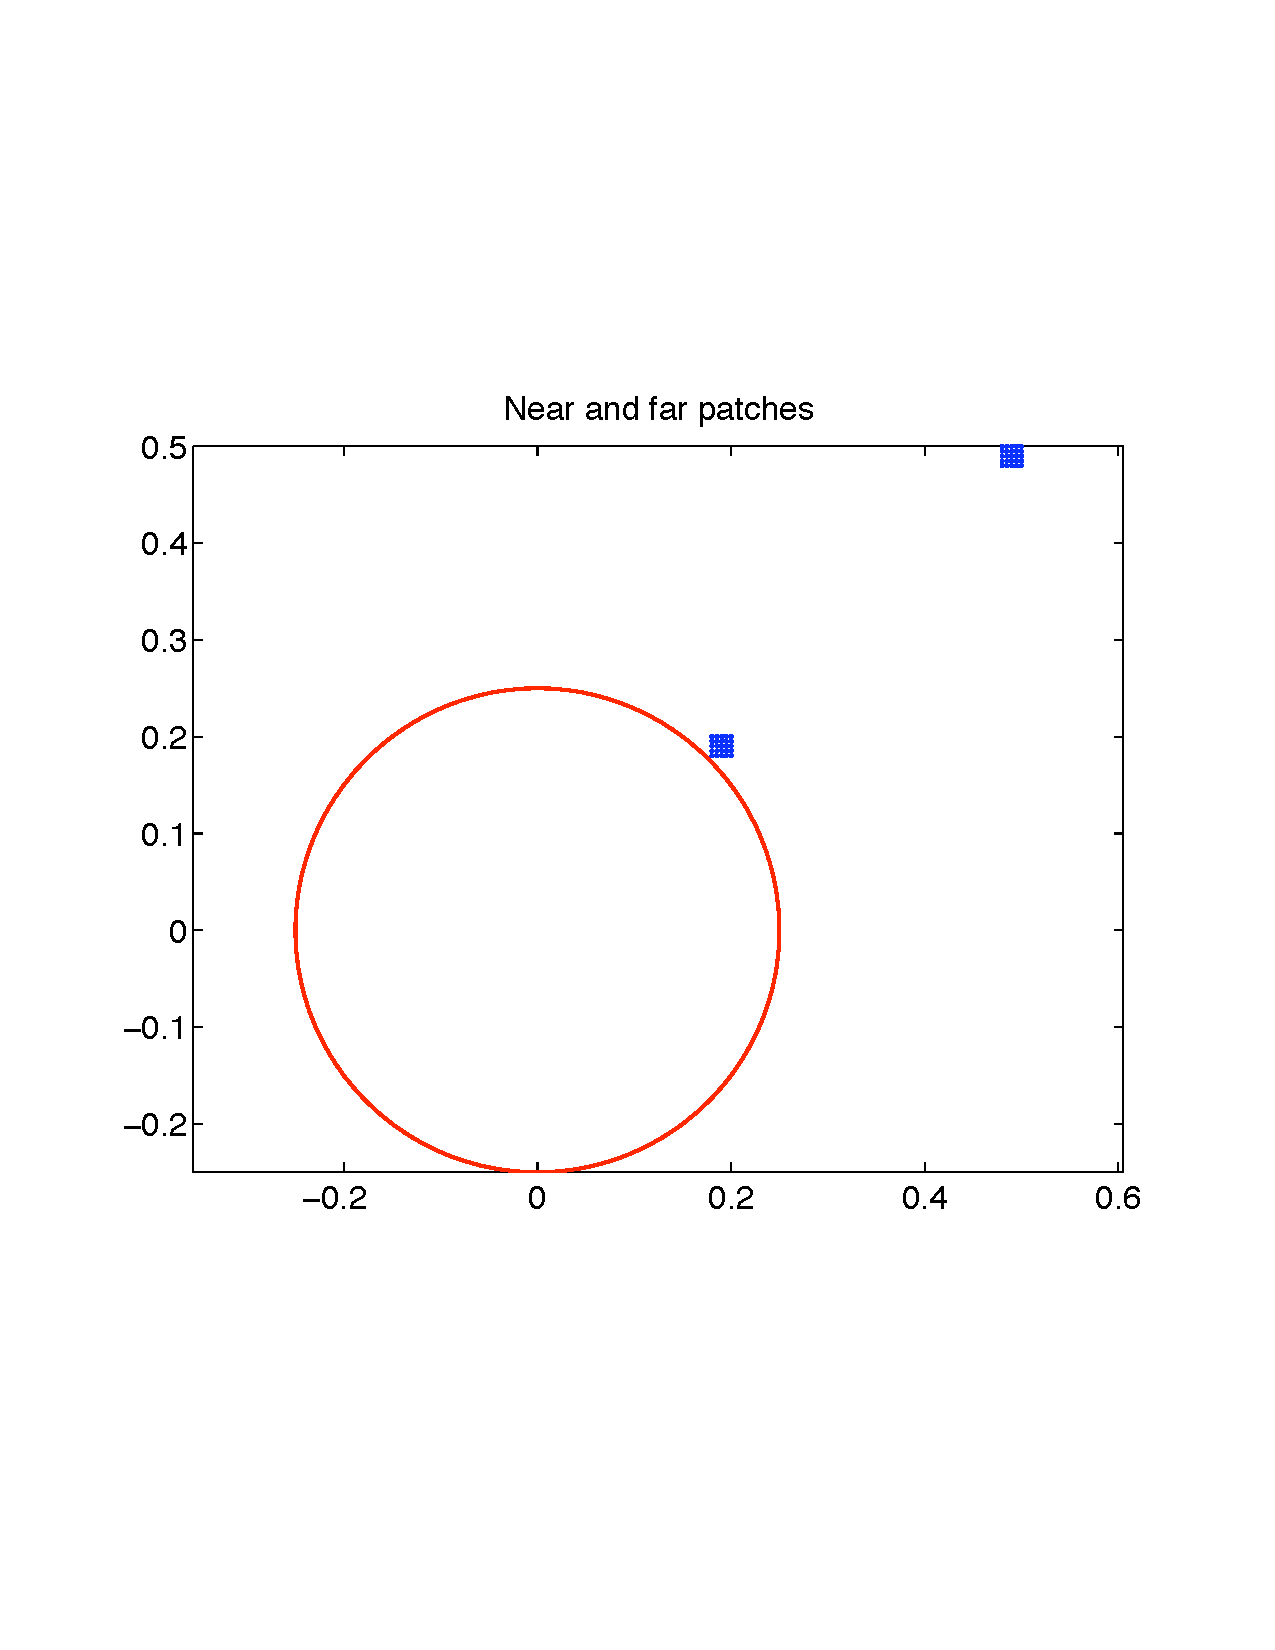
\includegraphics[width=3.0in]{StokesCylTest_farnearpatches_schematic.pdf}
\end{center}
\caption{The near and far patches on which the $L_2$ error is calculated.}
\label{schematic}
\end{figure}

We will also consider two different blob functions. One is from Cortez (2001):

\begin{eqnarray}\label{blob1}
	\phie(r) &=& \frac{3\eps^3}{2\pi\left( r^2 + \eps^2\right)^{5/2}} \nonumber \\
	\bu(\bx) &=& \frac{1}{4\pi\mu} \int_{\partial\Omega} -\ff(\by) \left[ \ln \left( \sqrt{r^2 + \eps^2} + \eps \right) - \frac{\eps\left( \sqrt{r^2 + \eps^2} + 2\eps \right)}{\left( \sqrt{r^2 + \eps^2} + \eps \right)\sqrt{r^2 + \eps^2}} \right] \nonumber \\
	&+& [\ff(\by) \cdot (\bx - \by)](\bx - \by)\left[  \frac{\sqrt{r^2 + \eps^2} + 2\eps}{\left( \sqrt{r^2 + \eps^2} + \eps \right)^2\sqrt{r^2 + \eps^2}} \right] \,\text{dS}(\by),
\end{eqnarray}
where $\phie$ is the blob function and the second equation is the integral formulation of the solution to Stokes flow that comes from using the blob instead of a $\delta$ function to find the fundamental solution. $\eps$ is a parameter controlling the spread of the blob, $r = \sqrt{\lvert \bx - \by \rvert}$, and $\partial\Omega$ is the domain boundary. The second blob has the advantage of a simpler kernel:
\begin{eqnarray}\label{blob2}
	\psie(r) &=& \frac{2\eps^4}{\pi\left( r^2 + \eps^2\right)^3} \nonumber \\
	\bu(\bx) &=& \frac{1}{8\pi\mu} \int_{\partial\Omega} -\ff(\by) \left[ \ln \left( \sqrt{r^2 + \eps^2} \right) - \frac{2\eps^2}{r^2 + \eps^2} \right] \nonumber \\
	&+& [\ff(\by) \cdot (\bx - \by)](\bx - \by)\left[  \frac{2}{r^2 + \eps^2} \right]\,\text{dS}(\by).
\end{eqnarray}

% [BEM methods with different M, trap vs hat]

First we look at the difference between the original method and a BEM with hat (or bilinear) basis functions and the trapezoidal rule with 50 points per chord. We plot error versus blob parameter value for $N=128$ in Fig.~\ref{errvsbp}. 

\begin{figure}[htp]
\begin{tabular}{cc}
	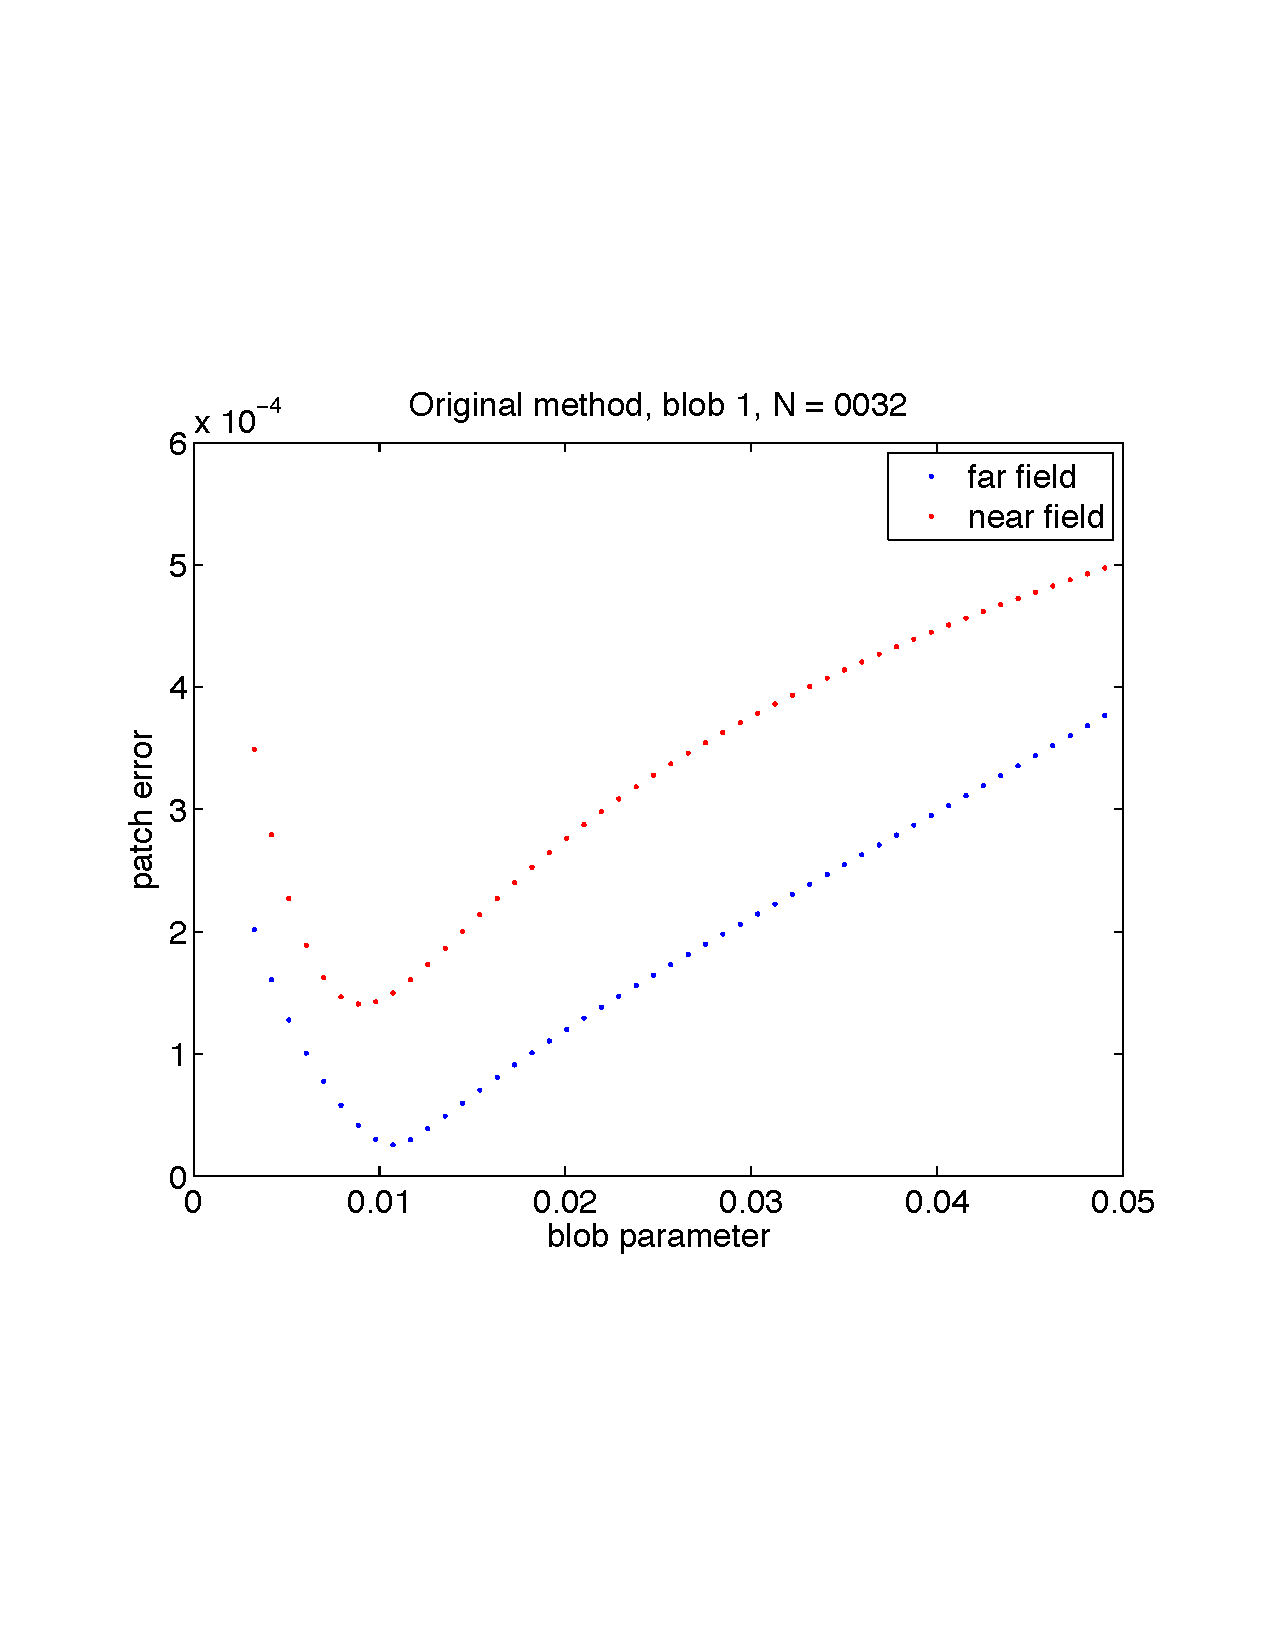
\includegraphics[width=3.75in]{StokesCylTest_compareBEMorig_bothblobs_origblob1N0032.pdf} & 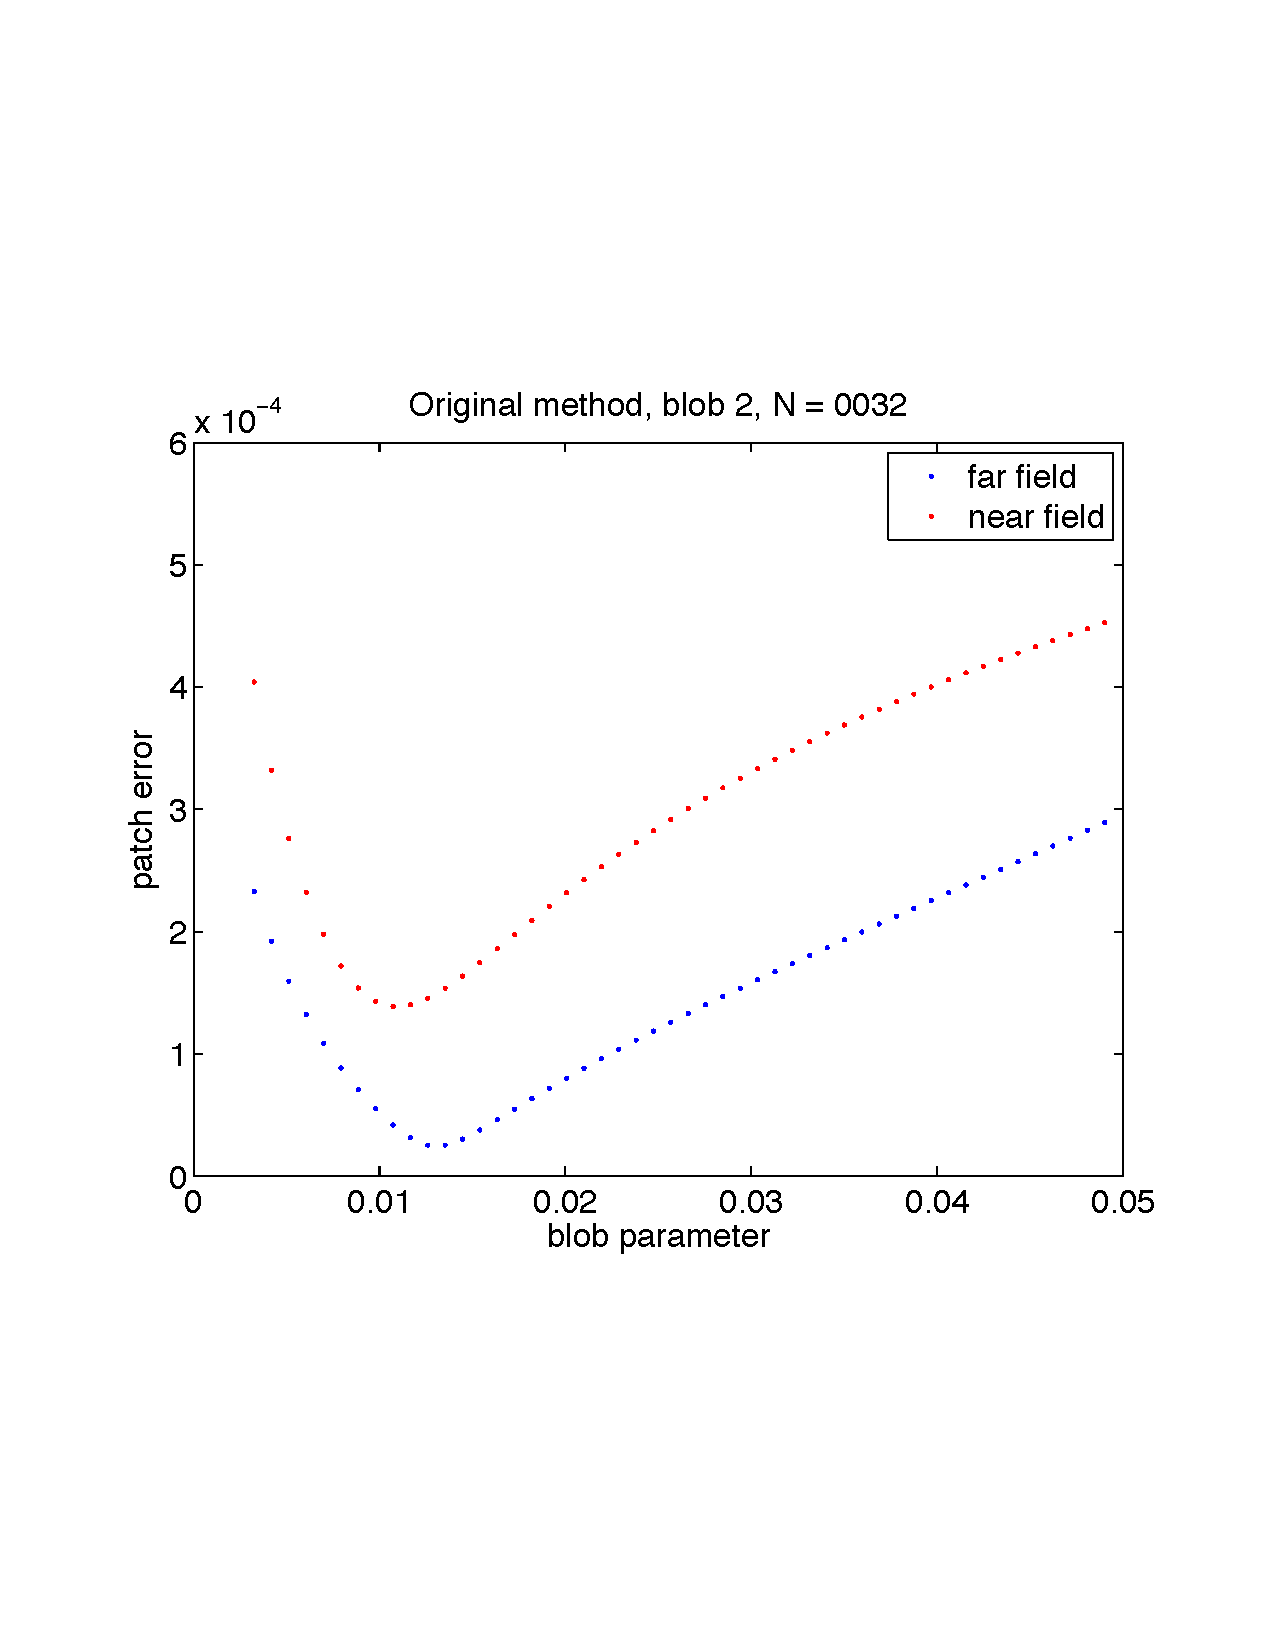
\includegraphics[width=3.75in]{StokesCylTest_compareBEMorig_bothblobs_origblob2N0032.pdf}\\
	A & B \\
	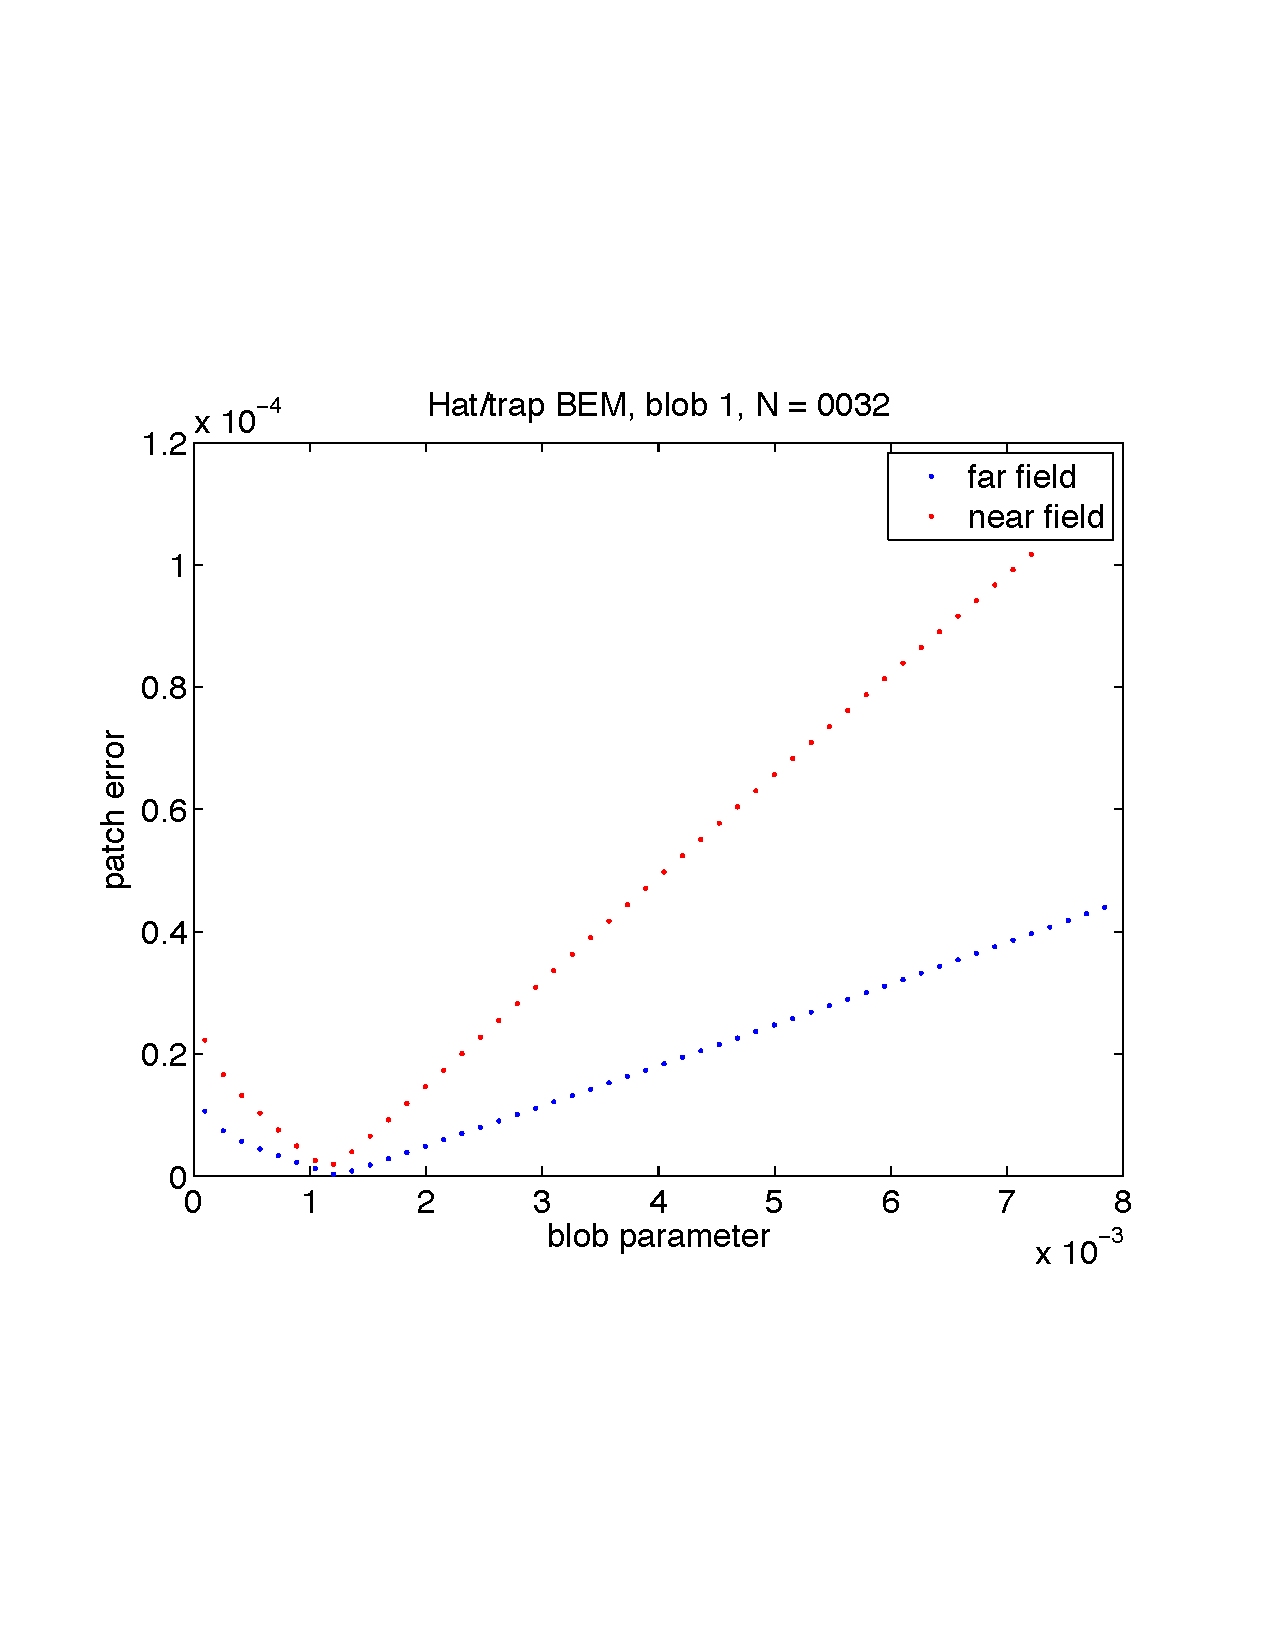
\includegraphics[width=3.75in]{StokesCylTest_compareBEMorig_bothblobs_hattrapblob1N0032.pdf} & 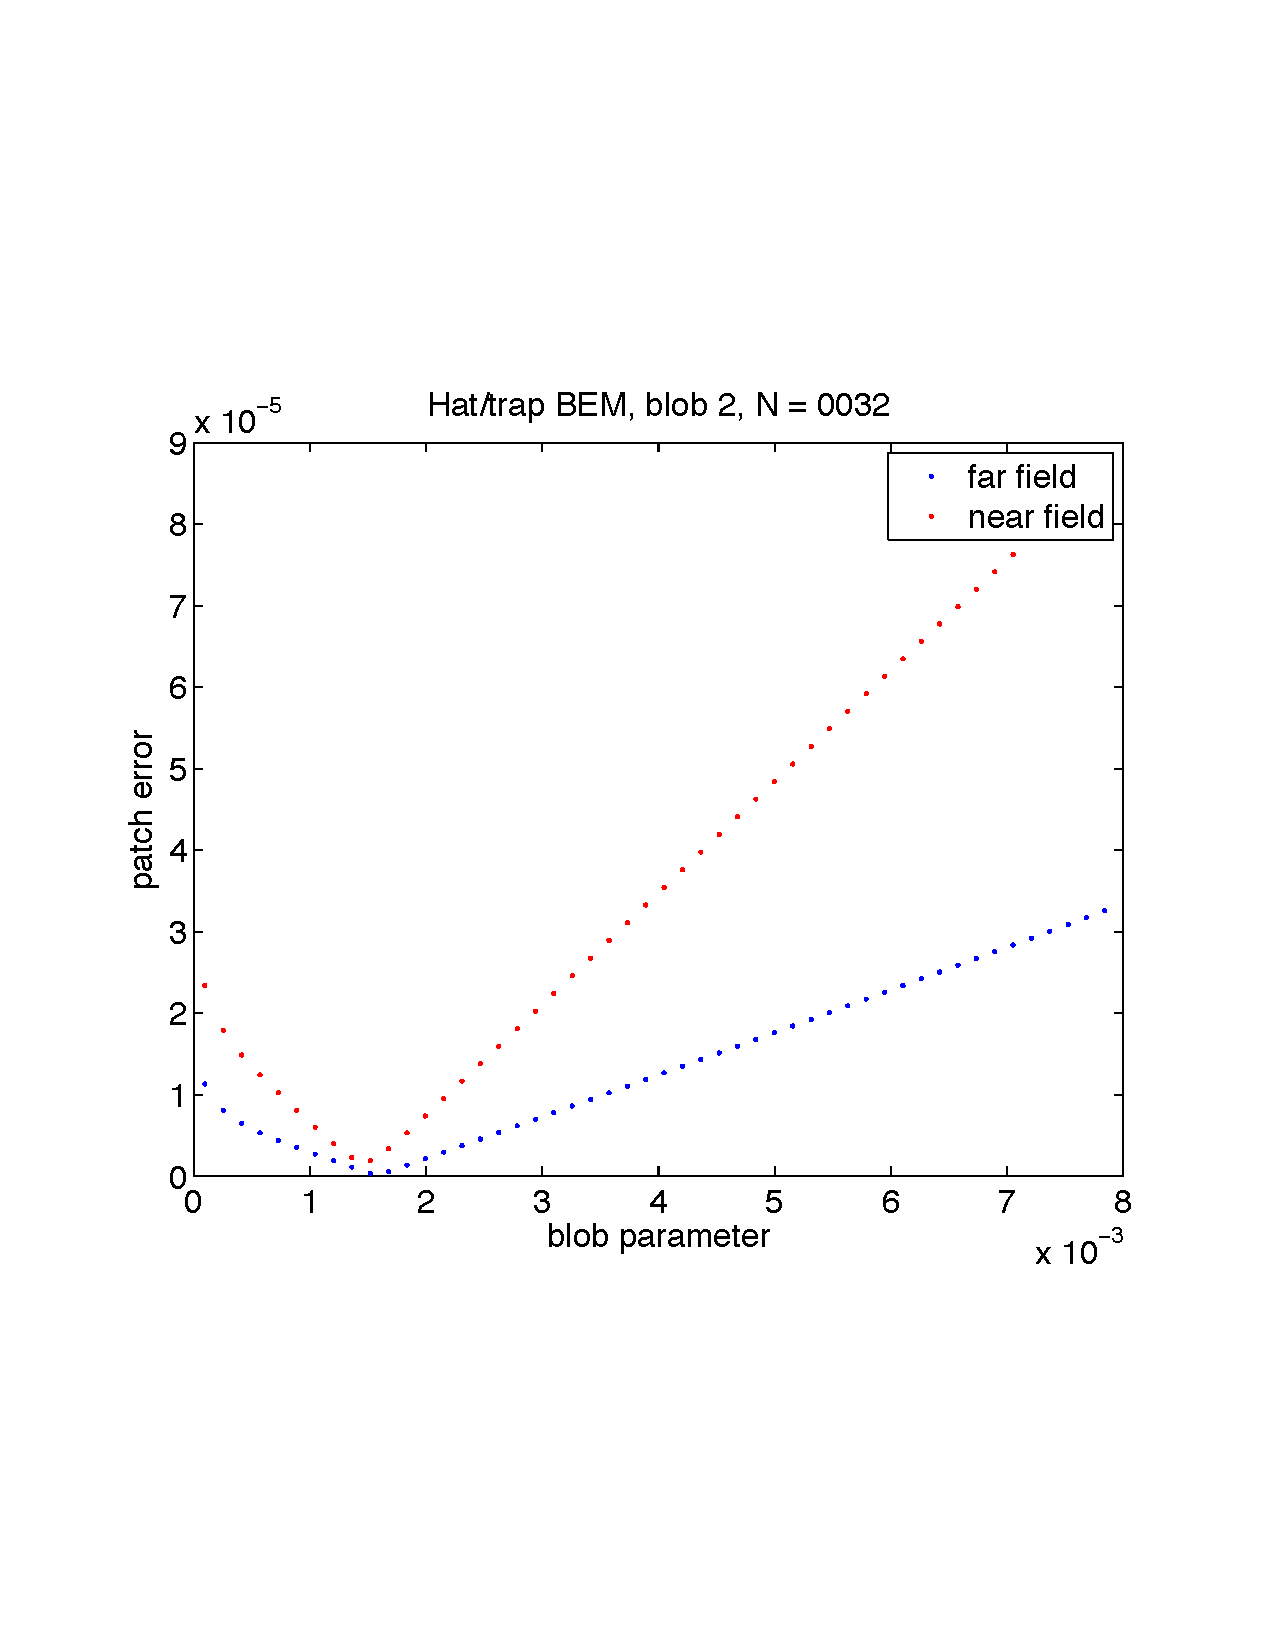
\includegraphics[width=3.75in]{StokesCylTest_compareBEMorig_bothblobs_hattrapblob2N0032.pdf}\\
	C & D
\end{tabular}
\caption{$L_2$ error vs blob parameter for the original and BEM methods at $N=32$ for the far and near patches and both blobs.}
\label{errvsbp}
\end{figure}



Then we consider the ideal blob size for the original method and the BEM based on the patch $L_2$ error. See Fig.~\ref{fig:idealblob} and Table~\ref{tab:idealblob}.

\begin{figure}[htp]
\begin{tabular}{cc}
	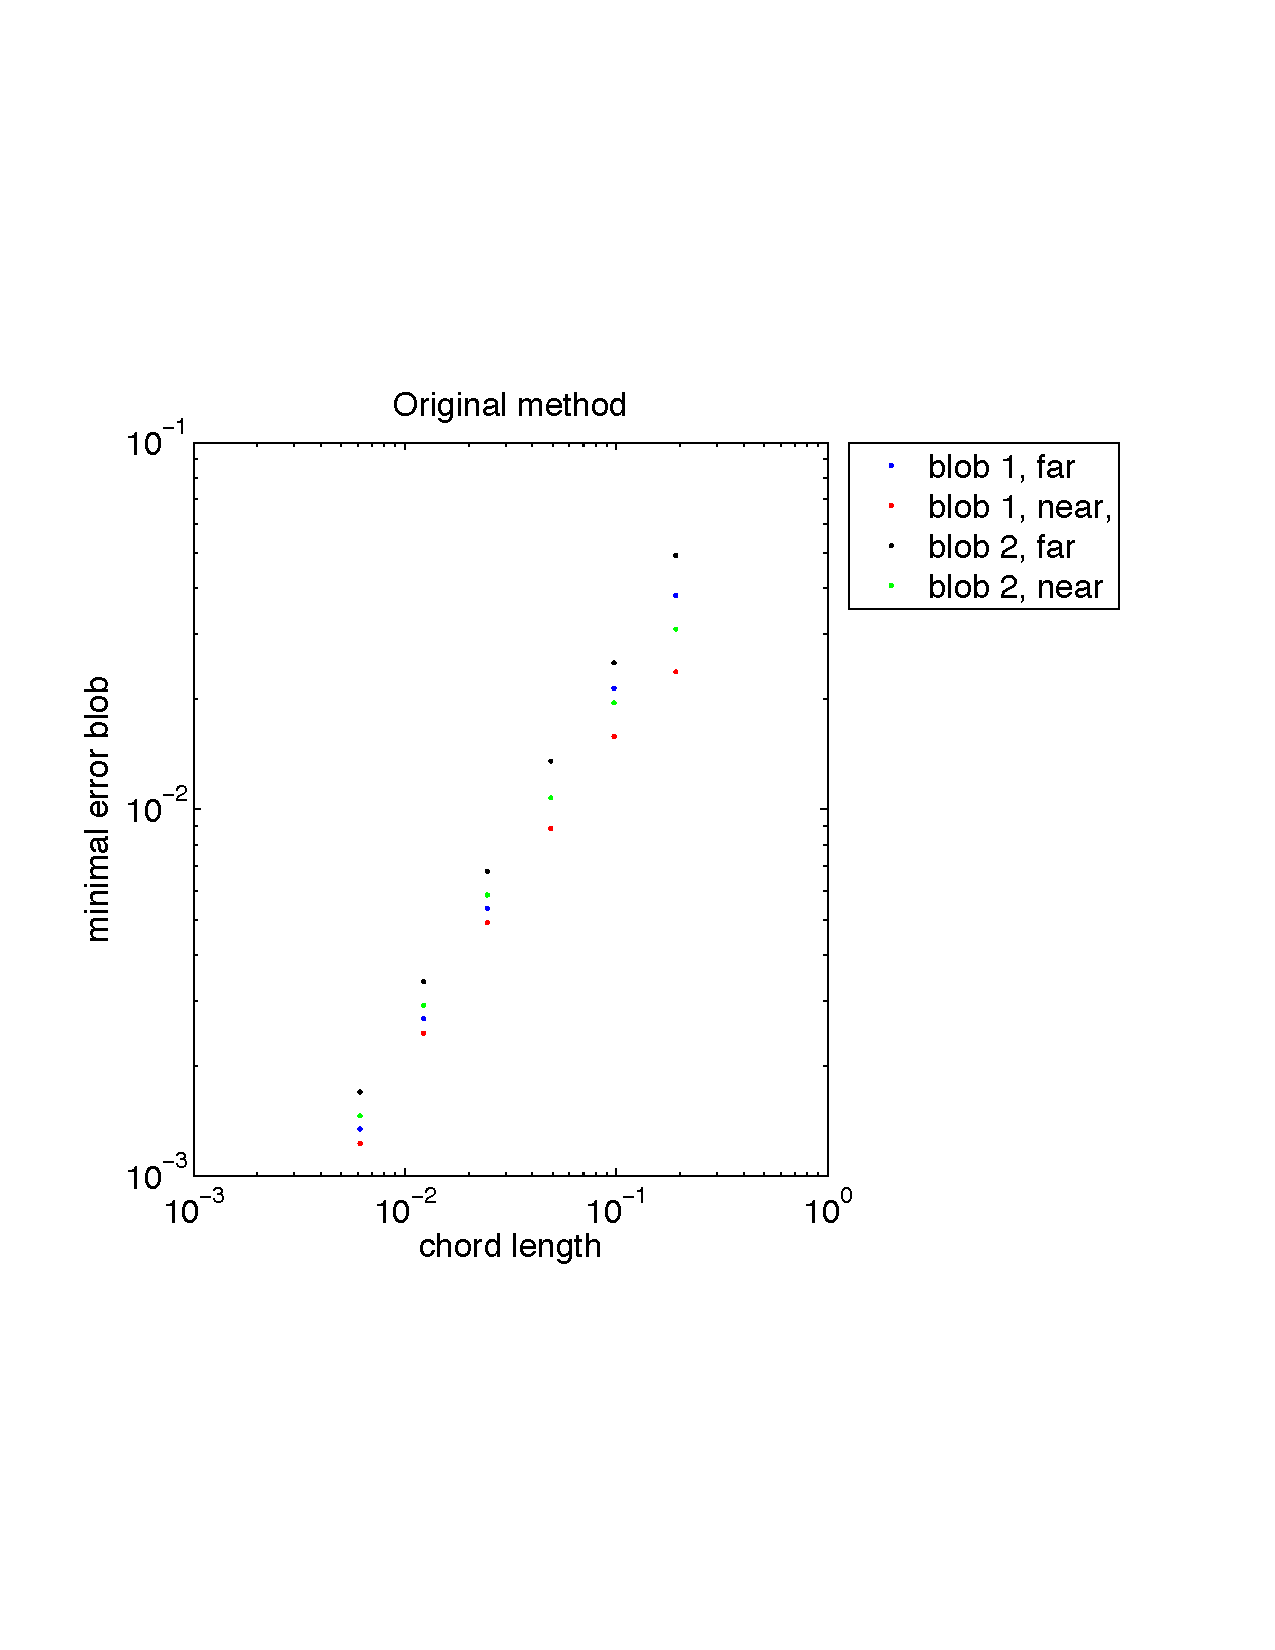
\includegraphics[width=3.75in]{StokesCylTest_compareBEMorig_bothblobs_idealbloborig.pdf} & 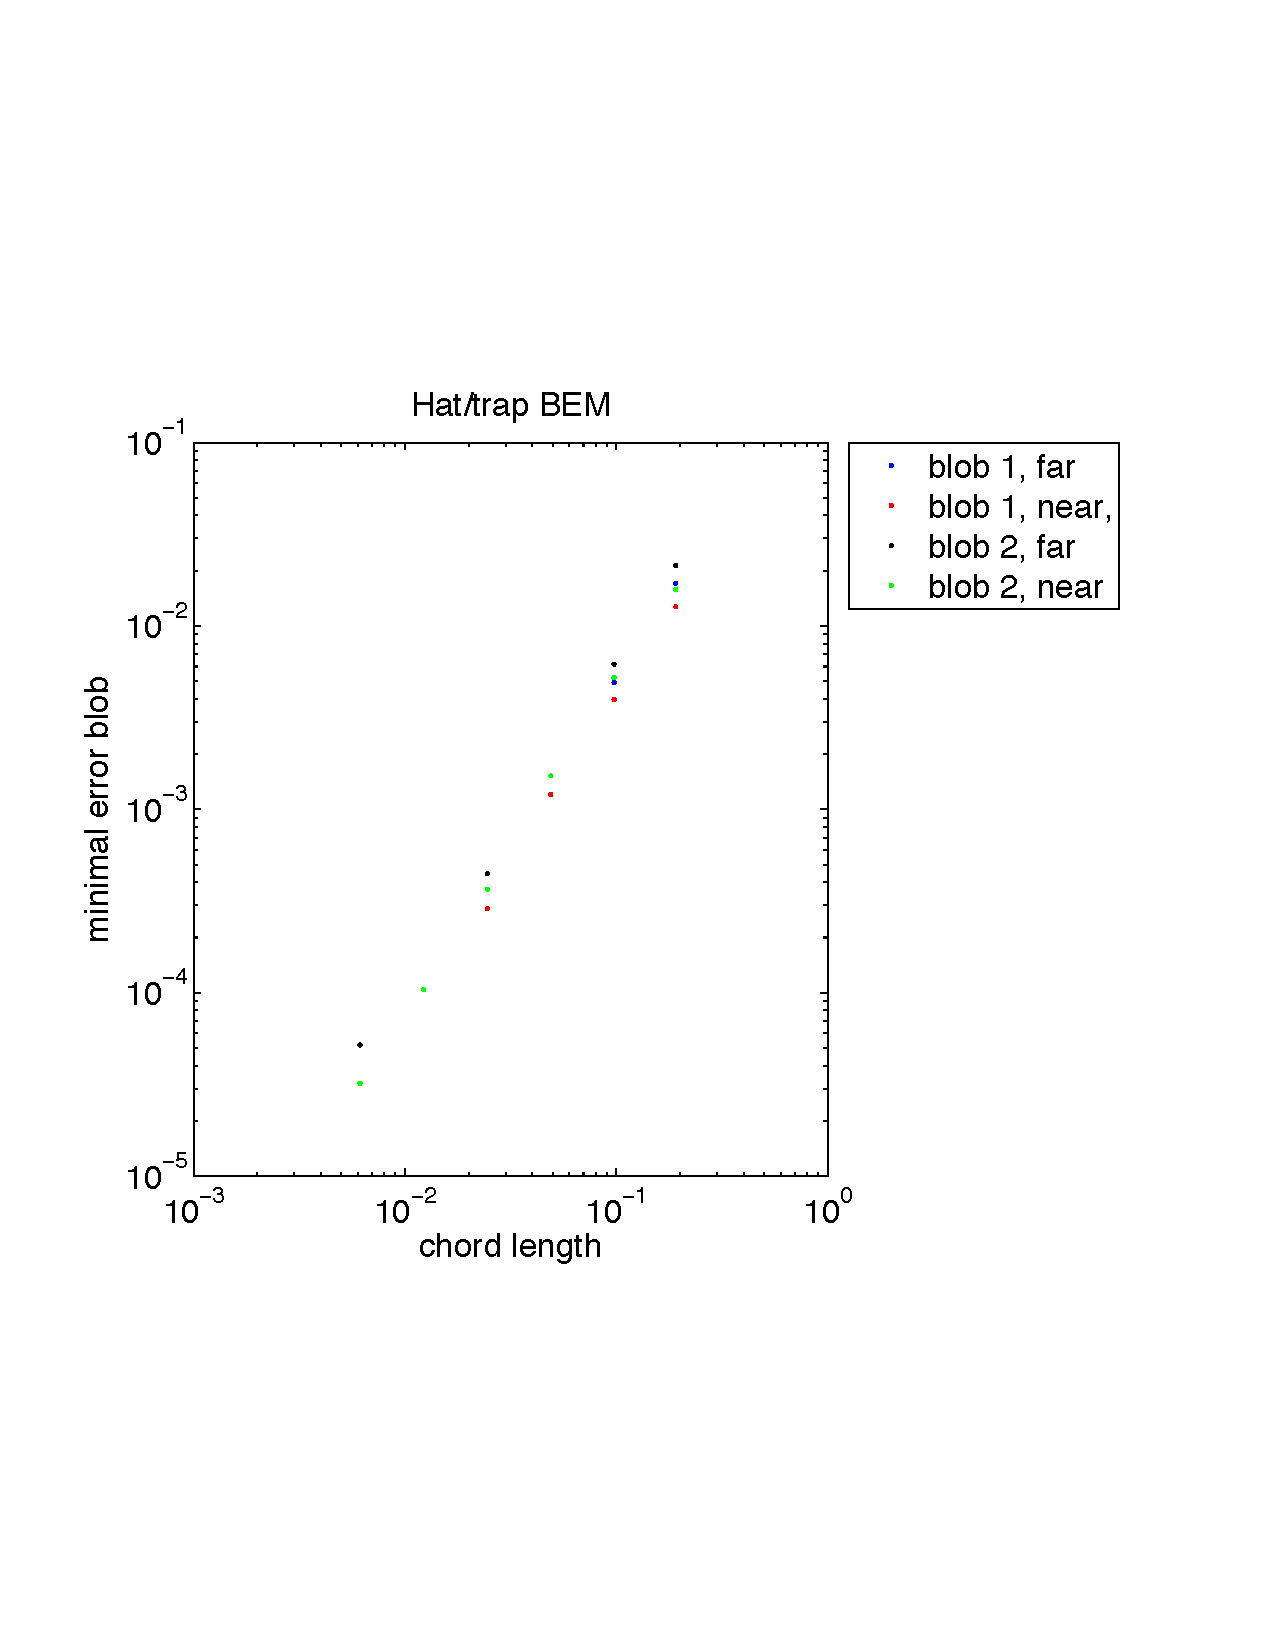
\includegraphics[width=3.75in]{StokesCylTest_compareBEMorig_bothblobs_idealblobBEM.pdf}\\
	A & B 
\end{tabular}
\caption{Ideal blob parameter versus chord length between nodes. Number of chords $N$ varies from 8 to 256. $M=50$ in the BEM.}
\label{fig:idealblob}
\end{figure}

\begin{table}[hbp]
	\centering
	\caption{The best fit $ax^b$ model of the dots in Fig.~\ref{fig:idealblob}.}
\begin{tabular}{|c|c|c|c|c|}
	\hline
	Method & Blob & Patch & Power $b$ & Coefficient $a$  \\
	\hline
	 \multirow{4}{*}{Original} & \multirow{2}{*}{Eq.~\ref{blob1}} &  Far   & 0.98124   &   0.20255  \\
      							& 								  & Near   & 0.87043   &   0.11333  \\
      							& \multirow{2}{*}{Eq.~\ref{blob2}} & Far   & 0.97632   &   0.24903  \\
      							& 								   & Near  & 0.89513   &   0.15026  \\
	 \multirow{4}{*}{Hat/trap BEM} & \multirow{2}{*}{Eq.~\ref{blob1}} &  Far   & 1.8409   &   0.33247  \\
      							& 								  & Near   & 1.7539   &   0.22804  \\
      							& \multirow{2}{*}{Eq.~\ref{blob2}} & Far   & 1.8078   &   0.38880  \\
      							& 								   & Near  & 1.8329   &   0.34974  \\
\hline
\end{tabular}\label{tab:idealblob}
\end{table}

\pagebreak
\section{Calculating exact integrals}

Let's try to find the exact integral values when we have linear hat elements over a chord using the second blob, integral shown again here for clarity:
%%%%%%%%%%%%%%%%%%%%%%%%%%%
\begin{eqnarray}\label{blob2uonly}
	\bu(\bx_*) &=& \frac{1}{4\pi\mu} \int_{\partial\Omega} -\ff(\bx) \left[ \frac{1}{2}\ln \left( r^2 + \eps^2 \right) - \frac{\eps^2}{r^2 + \eps^2} \right] \nonumber \\
	&+& [\ff(\bx) \cdot (\bx_* - \bx)](\bx_* - \bx)\left[  \frac{1}{r^2 + \eps^2} \right]\,d\ell(\bx) \nonumber \\
	\text{with   } r^2 &=& \lvert \bx_* - \bx \rvert^2.
\end{eqnarray}
%%%%%%%%%%%%%%%%%%%%%%%%%%%%
In the above equation, $\bx_* = (x_*,y_*)$ is the observation point and each $\bx = (x,y)$ is a pole on the boundary. 
If we define
%%%%%%%%%%%%%%%%%%%%%%%%%%%%%
\begin{eqnarray*}\label{defsformateqn}
	\Delta x &\equiv& x_* - x, \nonumber\\
	\Delta y &\equiv& y_* - y, \nonumber\\
	K_1(\bx) &\equiv& \frac{\eps^2}{r^2 + \eps^2} - \frac{1}{2}\ln\left(r^2 + \eps^2\right), \text{ and}\nonumber\\
	K_2(\bx) &\equiv& \frac{1}{r^2 + \eps^2},
\end{eqnarray*}
%%%%%%%%%%%%%%%%%%%%%%%%%%%%%%%%
we may rewrite Eq.~\eqref{blob2uonly} as a matrix equation:
%%%%%%%%%%%%%%%%%%%%%%%%%%%%%%%%%%
\begin{eqnarray}\label{mateqn}
	\bu(\bx_*) &=& \frac{1}{4\pi\mu} \int_{\partial\Omega} \begin{bmatrix} K_1(\bx) + K_2(\bx)(\Delta x)^2 & K_2(\bx) \Delta x \Delta y \\ K_2(\bx) \Delta x \Delta y & K_1(\bx) + K_2(\bx)(\Delta y)^2 \end{bmatrix} \ff(\bx)d\ell(\bx).
\end{eqnarray}
%%%%%%%%%%%%%%%%%%%%%%%%%%%%%%%%%%%

In the BEM, we discretize $\partial\Omega$ into $N$ equally spaced points and consider the linear segments, $S_k$, between the nodes $\bx_{k} = (x_{k},y_{k})$ and $\bx_{k+1} = (x_{k+1},y_{k+1})$ to be the elements in our method. Note that on a closed curve, $\bx_N$ coincides with $\bx_0$, resulting in $N$ chords, $S_0,\dotsc,S_{N-1}$; on an open curve $N$ points would result in $N-1$ chords. See Fig.~\ref{chordschematic} for examples.

\begin{figure}[h]
	\begin{center}
	\begin{tabular}{cc}
		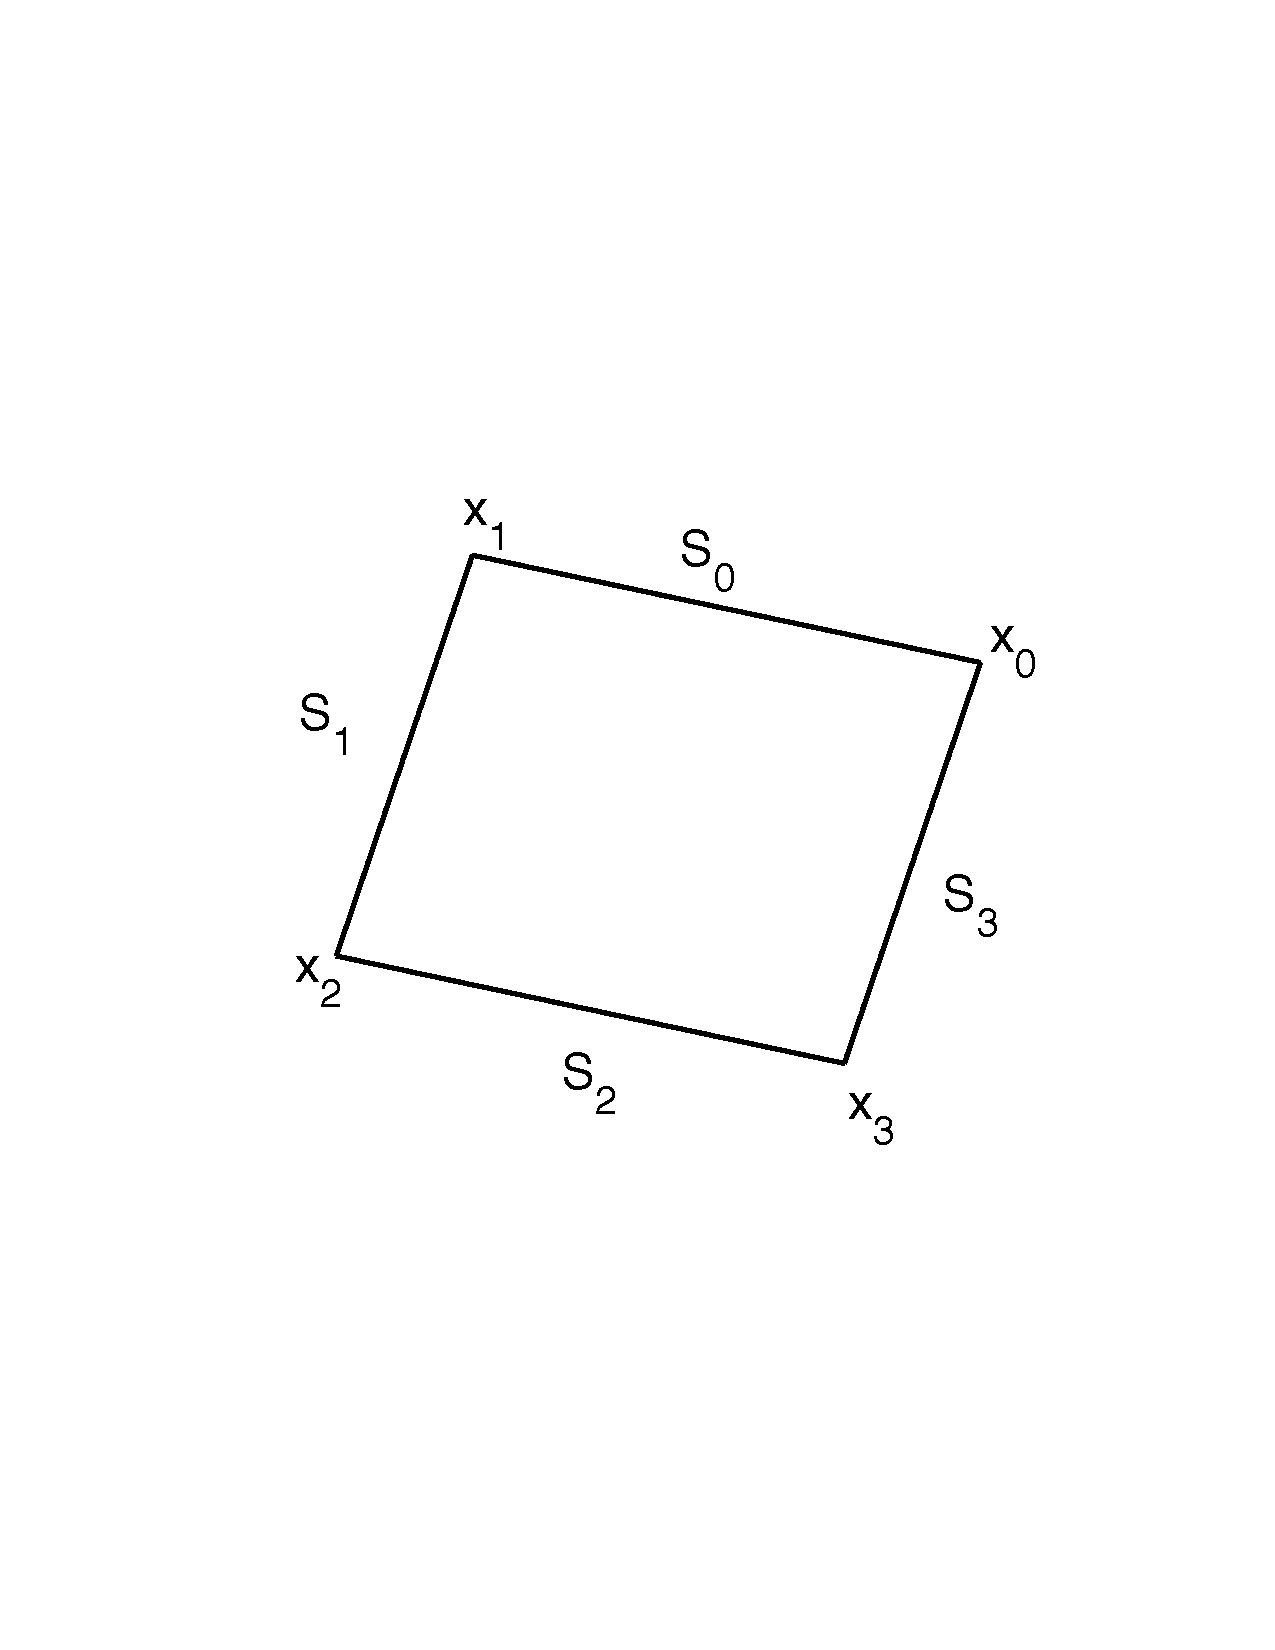
\includegraphics[width=3.0in]{chordschematic_closed.pdf} & 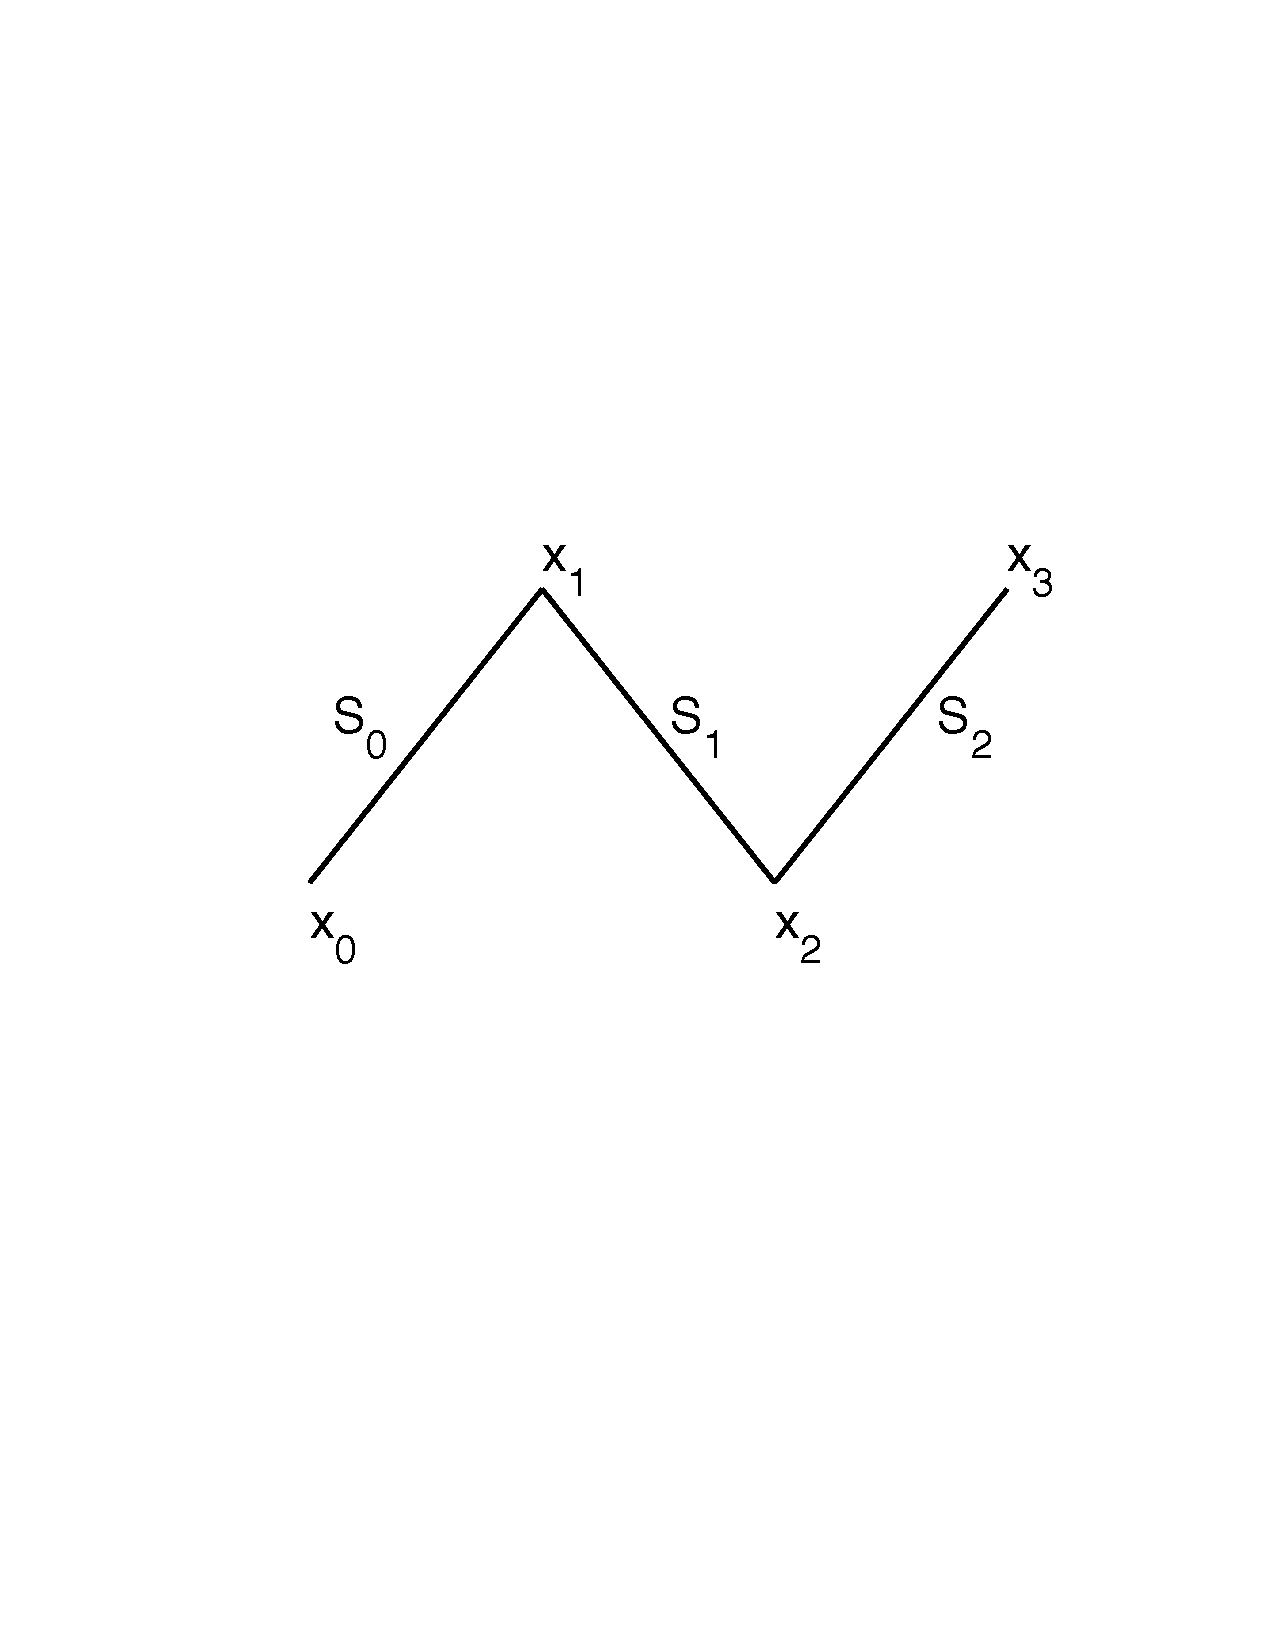
\includegraphics[width=3.0in]{chordschematic_open.pdf}
	\end{tabular}
\end{center}
	\caption{Indexing on discretized closed and open curves.}
	\label{chordschematic}
\end{figure}


On the $k$-th chord, the $x$ and $y$ coordinate functions may be given in terms of a parameter $s$:
%%%%%%%%%%%%%%%%%%%%%%%%%%%
\begin{eqnarray*}\label{xydefs}
	\hat{x}_k(s) &\equiv& (1-s)x_{k} + sx_{k+1} \text{ for } s \in [0,1] \text{ on } S_k , \nonumber\\
	\hat{y}_k(s) &\equiv& (1-s)y_{k} + sy_{k+1} \text{ for } s \in [0,1] \text{ on } S_k.
\end{eqnarray*}
%%%%%%%%%%%%%%%%%%%%%%%%%%%
We extend our earlier definitions to account for the discretization and parameterization:
%%%%%%%%%%%%%%%%%%%%%%%%%%%%%
\begin{eqnarray}\label{defsformateqnsdep}
	\Delta x_k(s) &\equiv& x_* - \hat{x}_k(s), \nonumber\\
	\Delta y_k(s) &\equiv& y_* - \hat{y}_k(s), \nonumber\\
	K_{1,k}(s) &\equiv& \frac{\eps^2}{r_k^2(s) + \eps^2} - \frac{1}{2}\ln\left(r_k^2(s) + \eps^2\right), \text{ and}\nonumber\\
	K_{2,k}(s) &\equiv& \frac{1}{r_k^2(s) + \eps^2}.
\end{eqnarray}
%%%%%%%%%%%%%%%%%%%%%%%%%%%%%%%%
We define linear basis functions over the chords to interpolate between the values of $\ff$ at the nodes $\bx_k$:
%%%%%%%%%%%%%%%%%%%%%%%%%%
\begin{eqnarray*}\label{BEMapprox}
	\ff(\bx) &\approx& \sum\limits_{k=0}^{N-1} \ff(\bx_k) \Phi_k(s), \nonumber \\
	\text{where } \Phi_k(s) &=& \left\{ \begin{array}{ll} s, & \text{ for } s \in [0,1] \text{ on } S_{k-1} \\  1 - s, & \text{ for } s \in [0,1] \text{ on } S_{k} \\ 0 & \text{ elsewhere} \end{array}\right.
\end{eqnarray*}
%%%%%%%%%%%%%%%%%%%%%%%%%%%%%
These approximations transform Eq.~\eqref{mateqn} into
%%%%%%%%%%%%%%%%%%%%%%%%%%%%%%%%%%
\begin{eqnarray}\label{BEMmateqn}
	\bu(\bx_*) &\approx& \frac{1}{4\pi\mu} \sum\limits_{k=0}^{N-1} \ff(\bx_k)^T \int_0^1 s \begin{bmatrix} K_{1,k-1}(s) + K_{2,k-1}(s)(\Delta x_{k-1}(s))^2 & K_{2,k-1}(s) \Delta x_{k-1}(s) \Delta y_{k-1}(s) \\ K_{2,k-1}(s) \Delta x_{k-1}(s) \Delta y_{k-1}(s) & K_{1,k-1}(s) + K_{2,k-1}(s)(\Delta y_{k-1}(s))^2 \end{bmatrix} \text{ds} \nonumber\\
	&+&  \frac{1}{4\pi\mu} \sum\limits_{k=0}^{N-1} \ff(\bx_k)^T \int_0^1 (1-s) \begin{bmatrix} K_{1,k}(s) + K_{2,k}(s)(\Delta x_{k}(s))^2 & K_{2,k}(s) \Delta x_{k}(s) \Delta y_{k}(s) \\ K_{2,k}(s) \Delta x_{k}(s) \Delta y_{k}(s) & K_{1,k}(s) + K_{2,k}(s)(\Delta y_{k}(s))^2 \end{bmatrix} \text{ds} \nonumber \\
	&\equiv& \frac{1}{4\pi\mu} \sum\limits_{k=0}^{N-1} \ff(\bx_k)^T\mathcal{M}^k.
\end{eqnarray}
%%%%%%%%%%%%%%%%%%%%%%%%%%%%%%%%%%%
Note that the above formulation holds for a closed curve. For an open curve with $N$ nodes and $N-1$ chords, the first summation occurs over $k=1,\dotsc,N-1$ and the second over $k=0,\dotsc,N-2$.

This is the formula for a single point. In reality, we will want to evaluate many points, and we will want to solve the matrix equation for the unknown forces $\ff$. For solving the integral equation, we will have the following:
\bees{
\bu(\bx_j) \approx \frac{1}{4\pi\mu} \sum\limits_{k=0}^{N-1} \ff(\bx_k)^T\mathcal{M}^{j,k},
}
where $\bu(\bx_j)$ is a known boundary condition at $\bx_j$ and $\mathcal{M}^{j,k}$ is $\mathcal{M}^{k}$ with the observation point $\bx_* = \bx_j$. In this manner we define a $2N$ by $2N$ matrix $\mathcal{M}$ composed of the 4 by 4 blocks $\mathcal{M}^{j,k}$. We will proceed with solving the matrix equation, although in order to evaluate velocities at points off the boundaries, the same procedures may be followed by simply replacing $\bx_j$ with $\bx_*$ as before.


We may rewrite the $\Delta x_k$ term as a quadratic:
%%%%%%%%%%%%%%%%%%%%%%%%%%%%%%%%
\begin{eqnarray*}\label{Dx}
	(\Delta x_{j,k}(s))^2 &=& (x_j - ((1-s)x_{k} + sx_{k+1}))^2 \nonumber \\
	&=& ((x_j - x_{k}) + s(x_{k} - x_{k+1}))^2 \nonumber \\
	&=& (x_j - x_{k})^2  + 2s(x_j - x_{k})(x_{k} - x_{k+1})+ s^2(x_{k} - x_{k+1})^2 \nonumber \\
	&\equiv& a_{0,j,k} + a_{1,j,k}s + a_{2,j,k}s^2.
\end{eqnarray*}
%%%%%%%%%%%%%%%%%%%%%%%%%%%%%%%%
Likewise,
%%%%%%%%%%%%%%%%%%%%%%%%%%%%%%%%
\begin{eqnarray*}\label{Dy}
	(\Delta y_{j,k}(s))^2 &=& (y_j - y_{k})^2  + 2s(y_j - y_{k})(y_{k} - y_{k+1})+ s^2(y_{k} - y_{k+1})^2 \nonumber \\
	&\equiv& b_{0,j,k} + b_{1,j,k}s + b_{2,j,k}s^2 \nonumber \\
	\Delta x_{j,k}(s)\Delta y_{j,k}(s) &=& ((x_j - x_{k}) + s(x_{k} - x_{k+1}))((y_j -y_{k}) + s(y_{k} - y_{k+1})) \nonumber \\ 
	&=& (x_j - x_{k})(y_j -y_{k}) + s\left((x_j - x_{k})(y_{k} - y_{k+1}) + (x_{k} - x_{k+1})(y_j -y_{k})\right) + s^2(x_{k} - x_{k+1})(y_{k} - y_{k+1}) \nonumber \\
	&\equiv& c_{0,j,k} + c_{1,j,k}s + c_{2,j,k}s^2.
\end{eqnarray*}
%%%%%%%%%%%%%%%%%%%%%%%%%%%%%%%%
With these quadratics and Eqs.~\eqref{defsformateqnsdep} and \eqref{BEMmateqn}, it can be seen that we need to perform integrations of the forms:
%%%%%%%%%%%%%%%%%%%%%%%%%%%%%%%%
\begin{eqnarray}\label{integraltypes}
	I_{1,k} &=& \int_0^1 \frac{1}{2}\ln\left(r_k^2(s) + \eps^2\right)\,\text{ds}  \nonumber \\
	I_{2,k} &=& \int_0^1 \frac{s}{2}\ln\left(r_k^2(s) + \eps^2\right)\;\text{ds}\nonumber \\   
	I_{3,k} &=& \int_0^1 \frac{1}{r_k^2(s) + \eps^2} \,\text{ds}\nonumber \\
	I_{4,k} &=& \int_0^1 \frac{s}{r_k^2(s) + \eps^2}\,\text{ds} \nonumber \\
	I_{5,k} &=& \int_0^1 \frac{s^2}{r_k^2(s) + \eps^2}\,\text{ds}  \nonumber \\
	I_{6,k} &=& \int_0^1 \frac{s^3}{r_k^2(s) + \eps^2}\;\text{ds}.
\end{eqnarray}
%%%%%%%%%%%%%%%%%%%%%%%%%%%%%%%%
Using this notation, 
%%%%%%%%%%%%%%%%%%%%%%%%%%%%%%%%%%
\begin{eqnarray}\label{Ks}
	\int_0^1 K_{1,k}(s) ds &=& \eps^2I_{3,k} - I_{1,k}\nonumber\\
	\int_0^1 sK_{1,k}(s) ds &=& \eps^2I_{4,k} - I_{2,k}\nonumber\\
	\int_0^1 K_{2,k}(s)(\alpha_0 + \alpha_1s + \alpha_2s^2) ds &=& \alpha_0I_{3,k} +\alpha_1I_{4,k}+\alpha_2I_{5,k}\nonumber\\
	\int_0^1 sK_{2,k}(s)(\alpha_0 + \alpha_1s + \alpha_2s^2) ds &=& \alpha_0I_{4,k} +\alpha_1I_{5,k}+\alpha_2I_{6,k}.
\end{eqnarray}
%%%%%%%%%%%%%%%%%%%%%%%%%%%%%%%%%%
Then the matrix acting on $\ff$ in Eq.~\ref{BEMmateqn} may be rewritten in component form as 
%%%%%%%%%%%%%%%%%%%%%%%%%%%%%%%%%%%%	
\begin{eqnarray}\label{BEMmatcomps}
	\mathcal{M}^{j,k}_{11} &=& \int_0^1 s K_{1,k-1} + sK_{2,k-1}(\Delta x_{j,k-1})^2 + K_{1,k} - sK_{1,k} + K_{2,k}(\Delta x_{j,k})^2 - sK_{2,k}(\Delta x_{j,k})^2 \\ 
	&=& \eps^2I_{4,k-1} - I_{2,k-1} + a_{0,j,k-1}I_{4,k-1} +a_{1,j,k-1}I_{5,k-1}+a_{2,j,k-1}I_{6,k-1} + \eps^2I_{3,k} - I_{1,k} + a_{0,j,k}I_{3,k} +a_{1,j,k}I_{4,k}+a_{2,j,k}I_{5,k}\nonumber \\ 
	&&-\left( \eps^2I_{4,k} - I_{2,k} + a_{0,j,k}I_{4,k} +a_{1,j,k}I_{5,k}+a_{2,j,k}I_{6,k} \right) \nonumber \\ 
	&=& -I_{2,k-1} + I_{4,k-1}\left(\eps^2 + a_{0,j,k-1} \right) + a_{1,j,k-1}I_{5,k-1} + a_{2,j,k-1}I_{6,k-1} \nonumber \\ 
	&&- I_{1,k}+ I_{2,k} + I_{3,k}\left(\eps^2 + a_{0,j,k} \right) + I_{4,k}\left(a_{1,j,k} - \eps^2 -a_{0,j,k}\right) + I_{5,k}(a_{2,j,k}-a_{1,j,k}) -a_{2,j,k}I_{6,k}\nonumber \\ 
	\mathcal{M}^{j,k}_{22} &=& -I_{2,k-1} + I_{4,k-1}\left(\eps^2 + b_{0,j,k-1} \right) + b_{1,j,k-1}I_{5,k-1} + b_{2,j,k-1}I_{6,k-1} \nonumber \\ 
	&&- I_{1,k}+ I_{2,k} + I_{3,k}\left(\eps^2 + b_{0,j,k} \right) + I_{4,k}\left(b_{1,j,k} - \eps^2 -b_{0,j,k}\right) + I_{5,k}(b_{2,j,k}-b_{1,j,k}) -b_{2,j,k}I_{6,k}\nonumber \\ 	
	\mathcal{M}^{j,k}_{12} &=& \int_0^1 s K_{2,k-1} \Delta x_{j,k-1} \Delta y_{j,k-1} + (1-s)K_{2,k} \Delta x_{j,k} \Delta y_{j,k} \\ 
	&=& c_{0,j,k-1}I_{4,k-1} +c_{1,j,k-1}I_{5,k-1}+c_{2,j,k-1}I_{6,k-1} + c_{0,j,k}I_{3,k} +I_{4,k}(c_{1,j,k}-c_{0,j,k})+I_{5,k}(c_{2,j,k}-c_{1,j,k}) -c_{2,j,k}I_{6,k} \nonumber \\ 
	\mathcal{M}^{j,k}_{21} &=& \mathcal{M}^{j,k}_{12}
\end{eqnarray}
%%%%%%%%%%%%%%%%%%%%%%%%%%%%%%%%%%%
In the case of an open curve, the $k=0$ block matrices, $\mathcal{M}^{j,0}$, will only have the $I_{i,k} = I_{i,1}$ terms and the $k=N-1$ matrices will only have the $I_{i,k-1} = I_{i,N-2}$ terms. All the other $\mathcal{M}^{j,k}$ remain the same. 

**Working on symmetry issues**

\subsection{The first integral: $I_{1,k} = \displaystyle{\int_0^1 \frac{1}{2}\ln\left(r_k^2(s) + \eps^2\right)}\, ds $}
We begin with the first integral in Eq.~\eqref{integraltypes}, by expanding $r_k^2(s) + \eps^2$.
%%%%%%%%%%%%%%%%%%%%%%%%%%%%%%%%
\begin{eqnarray}\label{r2}
	r_k^2(s)+ \eps^2 &=& \eps^2 + (\Delta x_k(s))^2 + (\Delta y_k(s))^2 \nonumber \\
	&=& \eps^2 + (a_{0,k} + a_{1,k}s + a_{2,k}s^2)  + (b_{0,k} + b_{1,k}s + b_{2,k}s^2)  \nonumber \\
	&\equiv& \eps^2 + r_{k-1}^2 + d_{1,k}s + h^2s^2,
\end{eqnarray}
%%%%%%%%%%%%%%%%%%%%%%%%%%%%%%%%
where $r_{k-1}^2 = \lvert \bx_* - \bx_{k-1} \rvert^2$ and $h^2 = \lvert \bx_{k} - \bx_{k-1} \rvert^2$ is the squared chord length, assumed to be the same for all $k$.

With this notation, the first integral becomes
%%%%%%%%%%%%%%%%%%%%%%%%%%%%%%%%
\begin{eqnarray*}\label{integral1}
	I_{1,k} &=& \int_0^1 \frac{\ln\left(\eps^2 + r_{k-1}^2 + d_{1,k}s + h^2s^2\right)}{2} \;ds.
\end{eqnarray*}
%%%%%%%%%%%%%%%%%%%%%%%%%%%%%%%%
Let $D_k$ be the discriminant of $r_k^2(s) + \eps^2$, $D_k \equiv d_{1,k}^2 - 4h^2(r_{k-1}^2+\eps^2)$. Since $r_k^2(s) + \eps^2 > 0$ for all choices of the observation point $\bx_*$ (including those on the boundary), $D_k < 0$ for all $\bx_*$. Because of this property, the following functions are well-defined over $\Omega\cup\partial\Omega$:
%%%%%%%%%%%%%%%%%%%%%%%%%%%%%
\begin{eqnarray*}\label{defsint}
	A_k(s) &\equiv& \arctan\left( \frac{d_{1,k} + 2h^2s}{\sqrt{-D_k}}\right), \nonumber\\
	L_k(s) &\equiv& \ln(r_k^2(s) + \eps^2).
\end{eqnarray*}
%%%%%%%%%%%%%%%%%%%%%%%%%%%%%%%%
It can be shown that $I_{1,k}$ is
%%%%%%%%%%%%%%%%%%%%%%%%%%%%%%%%%
\begin{eqnarray*}\label{integral1solved}
	I_{1,k} &=& -s + \frac{\sqrt{-D_k}}{2h^2}A_k(s) + \frac{d_{1,k} + 2h^2s}{4h^2}L_k(s) \bigg\vert_{s=0}^{s=1}. \end{eqnarray*}
%%%%%%%%%%%%%%%%%%%%%%%%%%%%%%%%%%
In the special case that $\bx_* = \bx_{k-1}$, several simplifications occur:
%%%%%%%%%%%%%%%%%%%%%%%%%%%%%%%%%%
\begin{eqnarray*}\label{speccase}
d_{1,k}&\rightarrow&0 \nonumber \\
r_{k-1}&\rightarrow&0 \nonumber \\
\sqrt{-D_k} &\rightarrow& 2h\eps \nonumber \\
A_k(s) &\rightarrow& \arctan(sh/\eps) \nonumber \\
L_k(s) &\rightarrow& \ln(h^2s^2 +\eps^2)
\end{eqnarray*}
%%%%%%%%%%%%%%%%%%%%%%%%%%%%%%%%%%
In this case, $I_{1,k}= -s + (\eps/h)\arctan(sh/\eps) + (s/2)\ln(h^2s^2 +\eps^2)\vert_0^1$.

\subsection{The second integral: $I_{2,k} = \displaystyle{\int_0^1 \frac{s}{2}\ln\left(r_k^2(s) + \eps^2\right)}\, ds $}
Using the notation in the previous section, it can be shown that 
%%%%%%%%%%%%%%%%%%%%%%%%%%%%%%%%%
\begin{eqnarray*}\label{integral2solved}
	I_{2,k} &=& \frac{1}{8h^4}\left[ 2h^2s(d_{1,k}-h^2s) - \left(2d_{1,k}\sqrt{-D_k}\right)A_k(s) +\left( -d_{1,k}^2 + 2h^2(\eps^2 + r_{k-1}^2 + h^2s^2)\right)L_k(s)  \right]_{s=0}^{s=1}. \end{eqnarray*}
%%%%%%%%%%%%%%%%%%%%%%%%%%%%%%%%%%
When $\bx_* = \bx_{k-1}$, $I_{2,k} = -s^2/4 + \left((h^2s^2+\eps^2)/4h^2\right)\ln(h^2s^2 +\eps^2)\vert_0^1$.

\subsection{The third integral: $I_{3,k} = \displaystyle{\int_0^1 \frac{1}{r_k^2(s) + \eps^2}}\, ds $}
%%%%%%%%%%%%%%%%%%%%%%%%%%%%%%%%%
\begin{eqnarray*}\label{integral3solved}
	I_{3,k} &=& \frac{2A_k(s)}{\sqrt{-D_k}}\bigg\vert_{s=0}^{s=1}. 
\end{eqnarray*}
%%%%%%%%%%%%%%%%%%%%%%%%%%%%%%%%%%
When $\bx_* = \bx_{k-1}$, $I_{3,k} = (1/\eps h)\arctan(h/\eps)$.

\subsection{The fourth integral: $I_{4,k} = \displaystyle{\int_0^1 \frac{s}{r_k^2(s) + \eps^2}}\, ds $}
%%%%%%%%%%%%%%%%%%%%%%%%%%%%%%%%%
\begin{eqnarray*}\label{integral4solved}
	I_{4,k} &=& \frac{1}{2h^2}L_k(s) - \frac{d_{1,k}}{h^2\sqrt{-D_k}}A_k(s)\bigg\vert_{s=0}^{s=1}. 
\end{eqnarray*}
%%%%%%%%%%%%%%%%%%%%%%%%%%%%%%%%%%
When $\bx_* = \bx_{k-1}$, $I_{4,k} = (1/2h^2)\ln(h^2s^2 +\eps^2)\vert_0^1$.

\subsection{The fifth integral: $I_{5,k} = \displaystyle{\int_0^1 \frac{s^2}{r_k^2(s) + \eps^2}}\, ds $}
%%%%%%%%%%%%%%%%%%%%%%%%%%%%%%%%%
\begin{eqnarray*}\label{integral5solved}
	I_{5,k} &=& \frac{s}{h^2} - \frac{d_{1,k}}{2h^4}L_k(s) + \frac{d_{1,k}^2 - 2h^2(r_{k-1}^2 + \eps^2)}{h^4\sqrt{-D_k}}A_k(s)\bigg\vert_{s=0}^{s=1}. 
\end{eqnarray*}
%%%%%%%%%%%%%%%%%%%%%%%%%%%%%%%%%%
When $\bx_* = \bx_{k-1}$, $I_{5,k} = s/h^2 - (2(r_{k-1}^2 + \eps^2)/h^2\sqrt{-D_k})\arctan(sh/\eps)\vert_0^1$.

\subsection{The sixth integral: $I_{6,k} = \displaystyle{\int_0^1 \frac{s^3}{r_k^2(s) + \eps^2}}\, ds $}
%%%%%%%%%%%%%%%%%%%%%%%%%%%%%%%%%
\begin{eqnarray*}\label{integral6solved}
	I_{6,k} &=& \frac{-d_{1,k}s}{h^4} + \frac{s^2}{2h^2} + \frac{d_{1,k}^2 - h^2(r_{k-1}^2 + \eps^2)}{2h^6}L_k(s) - \frac{d_{1,k}(d_{1,k}^2 - 3h^2(r_{k-1}^2 + \eps^2))}{h^6\sqrt{-D_k}}A_k(s)\bigg\vert_{s=0}^{s=1}. 
\end{eqnarray*}
%%%%%%%%%%%%%%%%%%%%%%%%%%%%%%%%%%
When $\bx_* = \bx_{k-1}$, $I_{6,k} = s^2/2h^2 - ((r_{k-1}^2 + \eps^2)/2h^4)\ln(h^2s^2 +\eps^2)\vert_0^1$.


\subsection{Numerical results}
Using Eq.~\eqref{BEMmatcomps} plus the values of the above six integrals, we construct the regularized Stokeslet matrix using exact integrals along each chord of the discretized domain. The next table compares the original method to the exact integral method over a range of  $N$-point discretizations of the circle, where $\eps = 2\pi/(5N)$ in the original method and $\eps = (2\pi/(5N))^2$ in the exact integral method. The first two sections of the table compare the $L_2$ error for far and near patches as described in the first section, while the second two consider only the error from a single near point, $0.26(\cos(0.7),\sin(0.7))$, and a single far point, $0.5(\cos(0.7),\sin(0.7))$. In both cases, the exact integral method converges as $h^2$ or better, while the original method converges as approximately $h$ (recall that $h$ is the chord length, which can be computed as $h = 0.25*2\sin(\pi/N)$).  [Might want to redo the table with better choices for $\eps$ (see poster). Also, switch to closer point 0.251.]

\pagebreak

\begin{center}
\begin{table}[htp]
	\begin{center}
\begin{tabular}{|l|l|l|l|l|l|}
	\hline
	\multicolumn{6}{|c|}{}\\
	\multicolumn{6}{|c|}{Original method, $L_2$ patch error, $\eps = 2\pi/(5N)$} \\
	\multicolumn{6}{|c|}{}\\
	\hline
	$N$ & $h$ & Far Patch Error & Far Patch Error/$h^{1.1}$ & Near Patch Error & Near Patch Error/$h^{1.1}$ \\
	\hline
	     8 & 0.19134  	&    0.001205  &   0.0074304   &   0.0034156  &   0.021061   \\
	    16 & 0.097545 	&  0.00051089  &     0.00661   &   0.0013597  &   0.017592   \\
	    32 & 0.049009 	&  0.00022611  &   0.0062376   &  0.00058368  &   0.016102   \\
	    64 & 0.024534 	&  0.00010486  &   0.0061925   &  0.00027706  &   0.016362   \\
	   128 & 0.012271 	&   5.025e-05  &   0.0063589   &  0.00013497  &    0.01708   \\
	   256 & 0.0061358	&  2.4562e-05  &    0.006662   &  6.6673e-05  &   0.018084   \\
							 	  														   
	\hline
	\multicolumn{6}{|c|}{}\\
	\multicolumn{6}{|c|}{Exact integral method, $L_2$ patch error, $\eps = (2\pi/(5N))^2$} \\
	\multicolumn{6}{|c|}{}\\
	\hline
	$N$ & $h$ & Far Patch Error & Far Patch Error/$h^2$ & Near Patch Error & Near Patch Error/$h^{2.5}$ \\
	\hline
	     8 & 0.19134  	&  1.9674e-05 &  0.00053738 &  0.00010273 & 0.0064149 \\
	    16 & 0.097545 	&  1.5585e-06 &   0.0001638 &  1.7096e-05 & 0.0057527 \\
	    32 & 0.049009 	&  2.8055e-07 &  0.00011681 &  2.0065e-06 & 0.0037736 \\
	    64 & 0.024534 	&  6.9671e-08 &  0.00011575 &  2.4804e-07 & 0.0026309 \\
	   128 & 0.012271 	&  1.8366e-08 &  0.00012198 &  4.0028e-08 & 0.0023999 \\
	   256 & 0.0061358	&  4.7773e-09 &  0.00012689 &  1.0788e-08 & 0.0036582 \\
							 	  														   
	\hline
	\multicolumn{6}{|c|}{}\\
	\multicolumn{6}{|c|}{Original method, $L_1$ point error, $\eps = 2\pi/(5N)$} \\
	\multicolumn{6}{|c|}{}\\
	\hline
	$N$ & $h$ & Far Point Error & Far Point Error/$h^{1.1}$ & Near Point Error & Near Point Error/$h$ \\
	\hline
	     8 & 0.19134  	&    0.079718   &   0.49155  &    0.17059   &   0.89154     \\
	    16 & 0.097545 	&    0.033907   &   0.43869  &   0.069224   &   0.70966     \\
	    32 & 0.049009 	&    0.015016   &   0.41426  &   0.028961   &   0.59093     \\
	    64 & 0.024534 	&   0.0069701   &   0.41162  &   0.011898   &   0.48495     \\
	   128 & 0.012271 	&   0.0033424   &   0.42297  &  0.0063705   &   0.51917     \\
	   256 & 0.0061358	&   0.0016345   &   0.44332  &  0.0031922   &   0.52025     \\
							 	  														   
	\hline
	\multicolumn{6}{|c|}{}\\
	\multicolumn{6}{|c|}{Exact integral method, $L_1$ point error, $\eps = (2\pi/(5N))^2$} \\
	\multicolumn{6}{|c|}{}\\
	\hline
	$N$ & $h$ & Far Point Error & Far Point Error/$h^{2.25}$ & Near Point Error & Near Point Error/$h^{2.5}$ \\
	\hline
	     8 & 0.19134  	&    0.0013932  &   0.057536 &   0.0032316   &   0.20179 \\
	    16 & 0.097545 	&   0.00015221  &   0.028623 &  0.00058728   &   0.19762 \\
	    32 & 0.049009 	&   2.4051e-05  &   0.021283 &  0.00018042   &   0.33932 \\
	    64 & 0.024534 	&   4.9607e-06  &   0.020824 &  1.2871e-05   &   0.13652 \\
	   128 & 0.012271 	&   1.2312e-06  &   0.024568 &  2.6067e-06   &   0.15629 \\
	   256 & 0.0061358	&   3.1698e-07  &   0.030083 &  5.1242e-07   &   0.17376 \\
							 	  														   
 \hline   
\end{tabular}
\end{center}
\end{table}
\end{center}	    
	    
	
	
\section{Calculating exact integrals over curves in 3D}

In three dimensions, we use the following blob function and associated Stokes' solution:
\baas{
\vphie(r) &=& \frac{15\eps^4}{8\pi(r^2+\eps^2)^{7/2}} \\
\bu(\bx_*) &=& \frac{1}{8\pi\mu} \int_{\partial\Omega} \ff(\bx)  \frac{r^2 + 2\eps^2}{\left( r^2 + \eps^2\right)^{3/2}} +  \frac{[\ff(\bx) \cdot (\bx_* - \bx)](\bx_* - \bx)}{\left( r^2 + \eps^2\right)^{3/2}} \,\text{d}\ell(\bx).
}
with $r = \lvert \bx_* - \bx \rvert$ as before. As in the previous section, we may write:
%%%%%%%%%%%%%%%%%%%%%%%%%%%%%%%%%%
\baas{
	\bu(\bx_*) &=& \frac{1}{8\pi\mu} \int_{\partial\Omega} \begin{bmatrix} K_1(r) + K_2(r)(\Delta x)^2 & K_2(r) \Delta x \Delta y & K_2(r) \Delta x \Delta z \\ K_2(r) \Delta x \Delta y & K_1(r) + K_2(r)(\Delta y)^2 & K_2(r) \Delta y \Delta z \\ K_2(r) \Delta x \Delta z & K_2(r) \Delta y \Delta z & K_1(r) + K_2(r)(\Delta z)^2 \end{bmatrix} \ff(\bx)d\ell(\bx),
}
%%%%%%%%%%%%%%%%%%%%%%%%%%%%%%%%%%%
where $\Delta z = z_* - z$ and 
%%%%%%%%%%%%%%%%%%%%%%%%%%%%%%%%%%
\baas{
K_1(r) &\equiv& \frac{r^2 + 2\eps^2}{\left(r^2 + \eps^2\right)^{3/2}}\\
K_2(r) &\equiv& \frac{1}{\left(r^2 + \eps^2\right)^{3/2}}.
}
%%%%%%%%%%%%%%%%%%%%%%%%%%%%%%%%%%%
After discretizing the boundary curve and approximating $\ff$ with linear basis functions as before, we have for a closed curve:
%%%%%%%%%%%%%%%%%%%%%%%%%%%%%%%%%%
\begin{eqnarray*}
	\bu(\bx_*) &\approx& \frac{1}{8\pi\mu} \sum\limits_{k=0}^{N-1} \ff(\bx_k)^T \int_0^1 s \begin{bmatrix} K_{1,k} + K_{2,k}(\Delta x_k)^2 & K_{2,k} \Delta x_k \Delta y_k & K_{2,k} \Delta x_k \Delta z_k \\ K_{2,k} \Delta x_k \Delta y_k & K_{1,k} + K_{2,k}(\Delta y_k)^2 & K_{2,k} \Delta y_k \Delta z_k \\ K_{2,k} \Delta x_k \Delta z_k & K_{2,k} \Delta y_k \Delta z_k & K_{1,k} + K_{2,k}(\Delta z_k)^2 \end{bmatrix} \text{ds} \nonumber\\
	&+&  \frac{1}{8\pi\mu} \sum\limits_{k=0}^{N-1} \ff(\bx_k)^T \int_0^1 (1-s) \begin{bmatrix} K_{1,k+1} + K_{2,k+1}(\Delta x_{k+1})^2 & K_{2,k+1} \Delta x_{k+1} \Delta y_{k+1} & K_{2,k+1} \Delta x_{k+1} \Delta z_{k+1} \\ K_{2,k+1} \Delta x_{k+1} \Delta y_{k+1} & K_{1,k+1} + K_{2,k+1}(\Delta y_{k+1})^2 & K_{2,k+1} \Delta y_{k+1} \Delta z_{k+1} \\ K_{2,k+1} \Delta x_{k+1} \Delta z_{k+1} & K_{2,k+1} \Delta y_{k+1} \Delta z_{k+1} & K_{1,k+1} + K_{2,k+1}(\Delta z_{k+1})^2 \end{bmatrix} \text{ds} \nonumber \\
	&\equiv& \frac{1}{8\pi\mu} \sum\limits_{k=0}^{N-1} \ff(\bx_k)^T\mathcal{M}^k,
\end{eqnarray*}
%%%%%%%%%%%%%%%%%%%%%%%%%%%%%%%%%%%
where for brevity we have suppressed the $s$ dependence in $K_1$, $K_2$, $\Delta x$, $\Delta y$, and $\Delta z$. As before, the formulation for an open curve may be achieved by changing the summation limits.

We may rewrite $r_k^2(s)+ \eps^2$ in terms of a quadratic in $s$:
%%%%%%%%%%%%%%%%%%%%%%%%%%%%%%%%
\begin{eqnarray}\label{3Dr2}
	r_k^2(s)+ \eps^2 &=& \eps^2 + (\Delta x_k(s))^2 + (\Delta y_k(s))^2 + (\Delta z_k(s))^2 \nonumber \\
	&=& \eps^2 + (a_{0,k} + a_{1,k}s + a_{2,k}s^2)  + (b_{0,k} + b_{1,k}s + b_{2,k}s^2) + (p_{0,k} + p_{1,k}s + p_{2,k}s^2) \nonumber \\
	&=& \eps^2 + (x_*-x_{k-1})^2 + (y_*-y_{k-1})^2 +(z_*-z_{k-1})^2 + (a_{1,k} + b_{1,k} + p_{1,k})s \nonumber\\
	&&+ \left((x_k-x_{k-1})^2 + (y_k-y_{k-1})^2 + (z_k-z_{k-1})^2\right)s^2 \nonumber \\
	&\equiv& \eps^2 + r_{k-1}^2 + d_{1,k}s + h^2s^2,
\end{eqnarray}
%%%%%%%%%%%%%%%%%%%%%%%%%%%%%%%%
where we denote the coefficients of the quadratic in $s$ of $\Delta z$ as $p_i$.
Then it is clear that we must perform the following types of integrations:
%%%%%%%%%%%%%%%%%%%%%%%%%%%%%%%%
\begin{eqnarray*}
	I_{1,k} &=& \int_0^1 \frac{1}{\left(r_k^2(s) + \eps^2\right)^{3/2}} \,\text{ds}\nonumber \\
	I_{2,k} &=& \int_0^1 \frac{s}{\left(r_k^2(s) + \eps^2\right)^{3/2}}\,\text{ds} \nonumber \\
	I_{3,k} &=& \int_0^1 \frac{s^2}{\left(r_k^2(s) + \eps^2\right)^{3/2}}\,\text{ds}  \nonumber \\
	I_{4,k} &=& \int_0^1 \frac{s^3}{\left(r_k^2(s) + \eps^2\right)^{3/2}}\;\text{ds},
\end{eqnarray*}
%%%%%%%%%%%%%%%%%%%%%%%%%%%%%%%%
since
\baas{
\int_0^1 K_{1,k}(s) ds &=& \left( 2\eps^2 + r_{k-1}^2 \right)I_{1,k} + d_{1,k}I_{2,k} + h^2I_{3,k}\\
\int_0^1 sK_{1,k}(s) ds &=& \left( 2\eps^2 + r_{k-1}^2 \right)I_{2,k} + d_{1,k}I_{3,k} + h^2I_{4,k}\\
\int_0^1 K_{2,k}(s)(\alpha_0 + \alpha_1s + \alpha_2s^2) ds &=& \alpha_0I_{1,k} +\alpha_1I_{2,k}+\alpha_2I_{3,k}\\
\int_0^1 sK_{2,k}(s)(\alpha_0 + \alpha_1s + \alpha_2s^2) ds &=& \alpha_0I_{2,k} +\alpha_1I_{3,k}+\alpha_2I_{4,k}.
}

The integrals can be solved (using Mathematica) to obtain
%%%%%%%%%%%%%%%%%%%%%%%%%%%%%%%%
\begin{eqnarray*}
	I_{1,k} &=& -\frac{2d_{1,k} + 4h^2s}{D_k \sqrt{r_k^2(s)+ \eps^2}}\Bigg|_{s=0}^{s=1} \\
	I_{2,k} &=& \frac{4r_{k-1}^2 + 2d_{1,k}s + 4\eps^2}{D_k \sqrt{r_k^2(s)+ \eps^2}}\Bigg|_{s=0}^{s=1}   \\
	I_{3,k} &=& -\frac{2d_{1,k}(\eps^2 + r_{k-1}^2) + 2s\left(d_{1,k}^2 -2h^2(\eps^2 + r_{k-1}^2)\right)}{h^2 D_k \sqrt{r_k^2(s)+ \eps^2}} + \frac{1}{h^3}\ln\left(d_{1,k}+2h^2s + 2h\sqrt{r_k^2(s)+ \eps^2}\right)\Bigg|_{s=0}^{s=1} \\
	I_{4,k} &=& -\frac{-s^2 h^2 D_k + s d_{1,k}\left( -3d_{1,k}^2 + 10h^2(\eps^2 + r_{k-1}^2)\right) + 8h^2(\eps^2 + r_{k-1}^2)^2 - 3d_{1,k}^2(\eps^2 + r_{k-1}^2)}{h^4 D_k \sqrt{r_k^2(s)+ \eps^2}} \\
	&& - \frac{3d_{1,k}}{2h^5}\ln\left( d_{1,k}+2h^2s + 2h\sqrt{r_k^2(s)+ \eps^2} \right)\Bigg|_{s=0}^{s=1}.
\end{eqnarray*}
%%%%%%%%%%%%%%%%%%%%%%%%%%%%%%%%
These functions are well-defined on $s \in [0,1]$. The only term where this is not entirely clear is $\ln\left( d_{1,k}+2h^2s + 2h\sqrt{r_k^2(s)+ \eps^2} \right)$. In order for this term to be well-defined, we require $d_{1,k}+2h^2s + 2h\sqrt{r_k^2(s)+ \eps^2} \equiv g'(s) + 2h\sqrt{g(s)}>0\;\;\forall\; s \in [0,1]$. Since $2h\sqrt{g(s)}>0\;\;\forall\; s \in [0,1]$, we are only interested in times when $g'(s) < 0$. The quadratic $g(s) \equiv r_k^2(s)+ \eps^2$ is concave up and so its smallest derivative will always occur at $s=0$. Plugging in $s=0$, our constraint reduces to $d_{1,k} + 2h\sqrt{\eps^2 + r_{k-1}^2} >0\;\;\forall\; s \in [0,1]$, which is always true since the discriminant is strictly less than zero: $D_k = d_{1,k}^2 - 4h^2(r_{k-1}^2+\eps^2) < 0$.

Using these formulas, we may the write the 3D regularized Stokeslet matrix as
\baas{
\mathcal{M}^k_{11} &=& \int_0^1 s K_{1,k} + sK_{2,k}(\Delta x_k)^2 + K_{1,k+1} - sK_{1,k+1} + K_{2,k+1}(\Delta x_k)^2 - sK_{2,k+1}(\Delta x_k)^2 \\
				   &=& \left( 2\eps^2 + r_{k-1}^2 \right)I_{2,k} + d_{1,k}I_{3,k} + h^2I_{4,k} + a_0I_{1,k} +a_1I_{2,k}+a_2I_{3,k} + 
}



\section{Calculating exact integrals for Brinkmanlets}

The Brinkman equations (or the unsteady Stokes equations forced at one frequency) can be regularized as well. In three dimensions, the blob function and associated velocity field are:
\baas{
\zeta_{\eps}(r) &=& \frac{(r+2\eps)^2}{224\pi\eps^5}e^{-r/\eps} \\
\bu(\bx_*) &=& \frac{1}{8\pi\mu} \int_{\partial\Omega} -\ff(\bx) \frac{rB''_\eps + B'_\eps}{r} + [\ff(\bx) \cdot (\bx_* - \bx)](\bx_* - \bx) \frac{rB''_\eps - B'_\eps}{r^3} d\bx\\
B_\eps(r) &=& \frac{1 - e^{-r/\eps}}{4\pi\lambda^2r} + \frac{\lambda^2\eps^2 - 7}{28\pi\lambda^2(\lambda^2\eps^2 - 1)^4}\frac{e^{-\lambda r} - e^{-r/\eps}}{r} \\
&& - \frac{\eps e^{-r/\eps}}{224\pi(\lambda^2\eps^2 -1)} \left[ r^2/\eps^2 + \frac{2(5\lambda^2\eps^2 - 8)}{\lambda^2\eps^2 - 1}r/\eps + \frac{2(19\lambda^4\eps^4 - 55\lambda^2\eps^2 + 48)}{\lambda^2\eps^2 - 1}  \right],
}
where primes denote derivatives with respect to $r$, and $\lambda$ is the constant in the nondimensional Brinkman equation: $(\nabla^2 - \lambda^2) \bu = \nabla p - \ff\zeta_{\eps}(r)$. In Brinkman flow, $\lambda^2$ is a real number. When considering the unsteady Stokes equations in a single frequency $\omega$, $\lambda^2$ is the imaginary number $i\omega/\nu$, where $\nu$ is the kinematic viscosity of the fluid. In order to know what integrals to solve, we must find the derivatives of $B_\eps$.







 
 
 
 
 
 
	    
	    
	    
    




  	























\end{document}





